\documentclass[onecolumn]{preport}

\usepackage[dvipdfmx]{graphicx}
\usepackage{comment}


\graphicspath{{figs/}}

\title{2021年度 SPIN:\\
Development and  of Iron Thin Films for Polarization Analysis of Ultracold Neutrons}
\author{Hiroaki Akatsuka }

\begin{document}
\pagestyle{empty}
\maketitle
\thispagestyle{empty}
\sloppy

%\part{Contents}
\section{abstract}
TUCAN実験では、中性子電気双極子モーメント(nEDM)の探索を目指している。nEDMの大きさは中性子の偏極度を測定することで求められる。我々は、中性子の偏極度を測定する、Simultaneous Spin Analyzer (SSA)を開発している\cite{SSA}。SSAではスピン解析に、磁化した鉄薄膜を用いる。この鉄薄膜は、十分に小さい磁場の印加によって飽和すること、薄膜中でスピン状態の異なる中性子が感じるポテンシャル差が大きいことが要求される。本文では、開発した鉄薄膜について、磁気特性を評価した結果について報告する。


\section{Introduction}

\subsection{Background}
超冷中性子(UCN)は、エネルギーが$\sim 100 \,\rm eV$以下の非常に遅い中性子である。そのため、UCNは特定の物質の表面で全反射し、閉じ込めることができる。この性質を生かして、UCNは中性子電気双極子モーメント(nEDM)探索、中性子寿命測定、重力実験などに用いられている。これらの実験のためには、高いUCN密度が必要となり、大強度UCN源の開発が進められている。TUCAN(TRIUMF Ultra-Cold Advanced Neu-tron)コラボレーションでは、TRIUMFの陽子専用ビームラインでnEDM探索実験に向けた大強度UCN源の開発を行っている。現在のnEDMの上限値は$1.8\times10^{-26}\,\rm e\cdot cm $ \cite{PSI}であり、我々は$10^{-27}\,\rm e\cdot cm ecm$の感度を達成することを目標としている。

\begin{comment}
\begin{figure}[tbh]
 \centering
 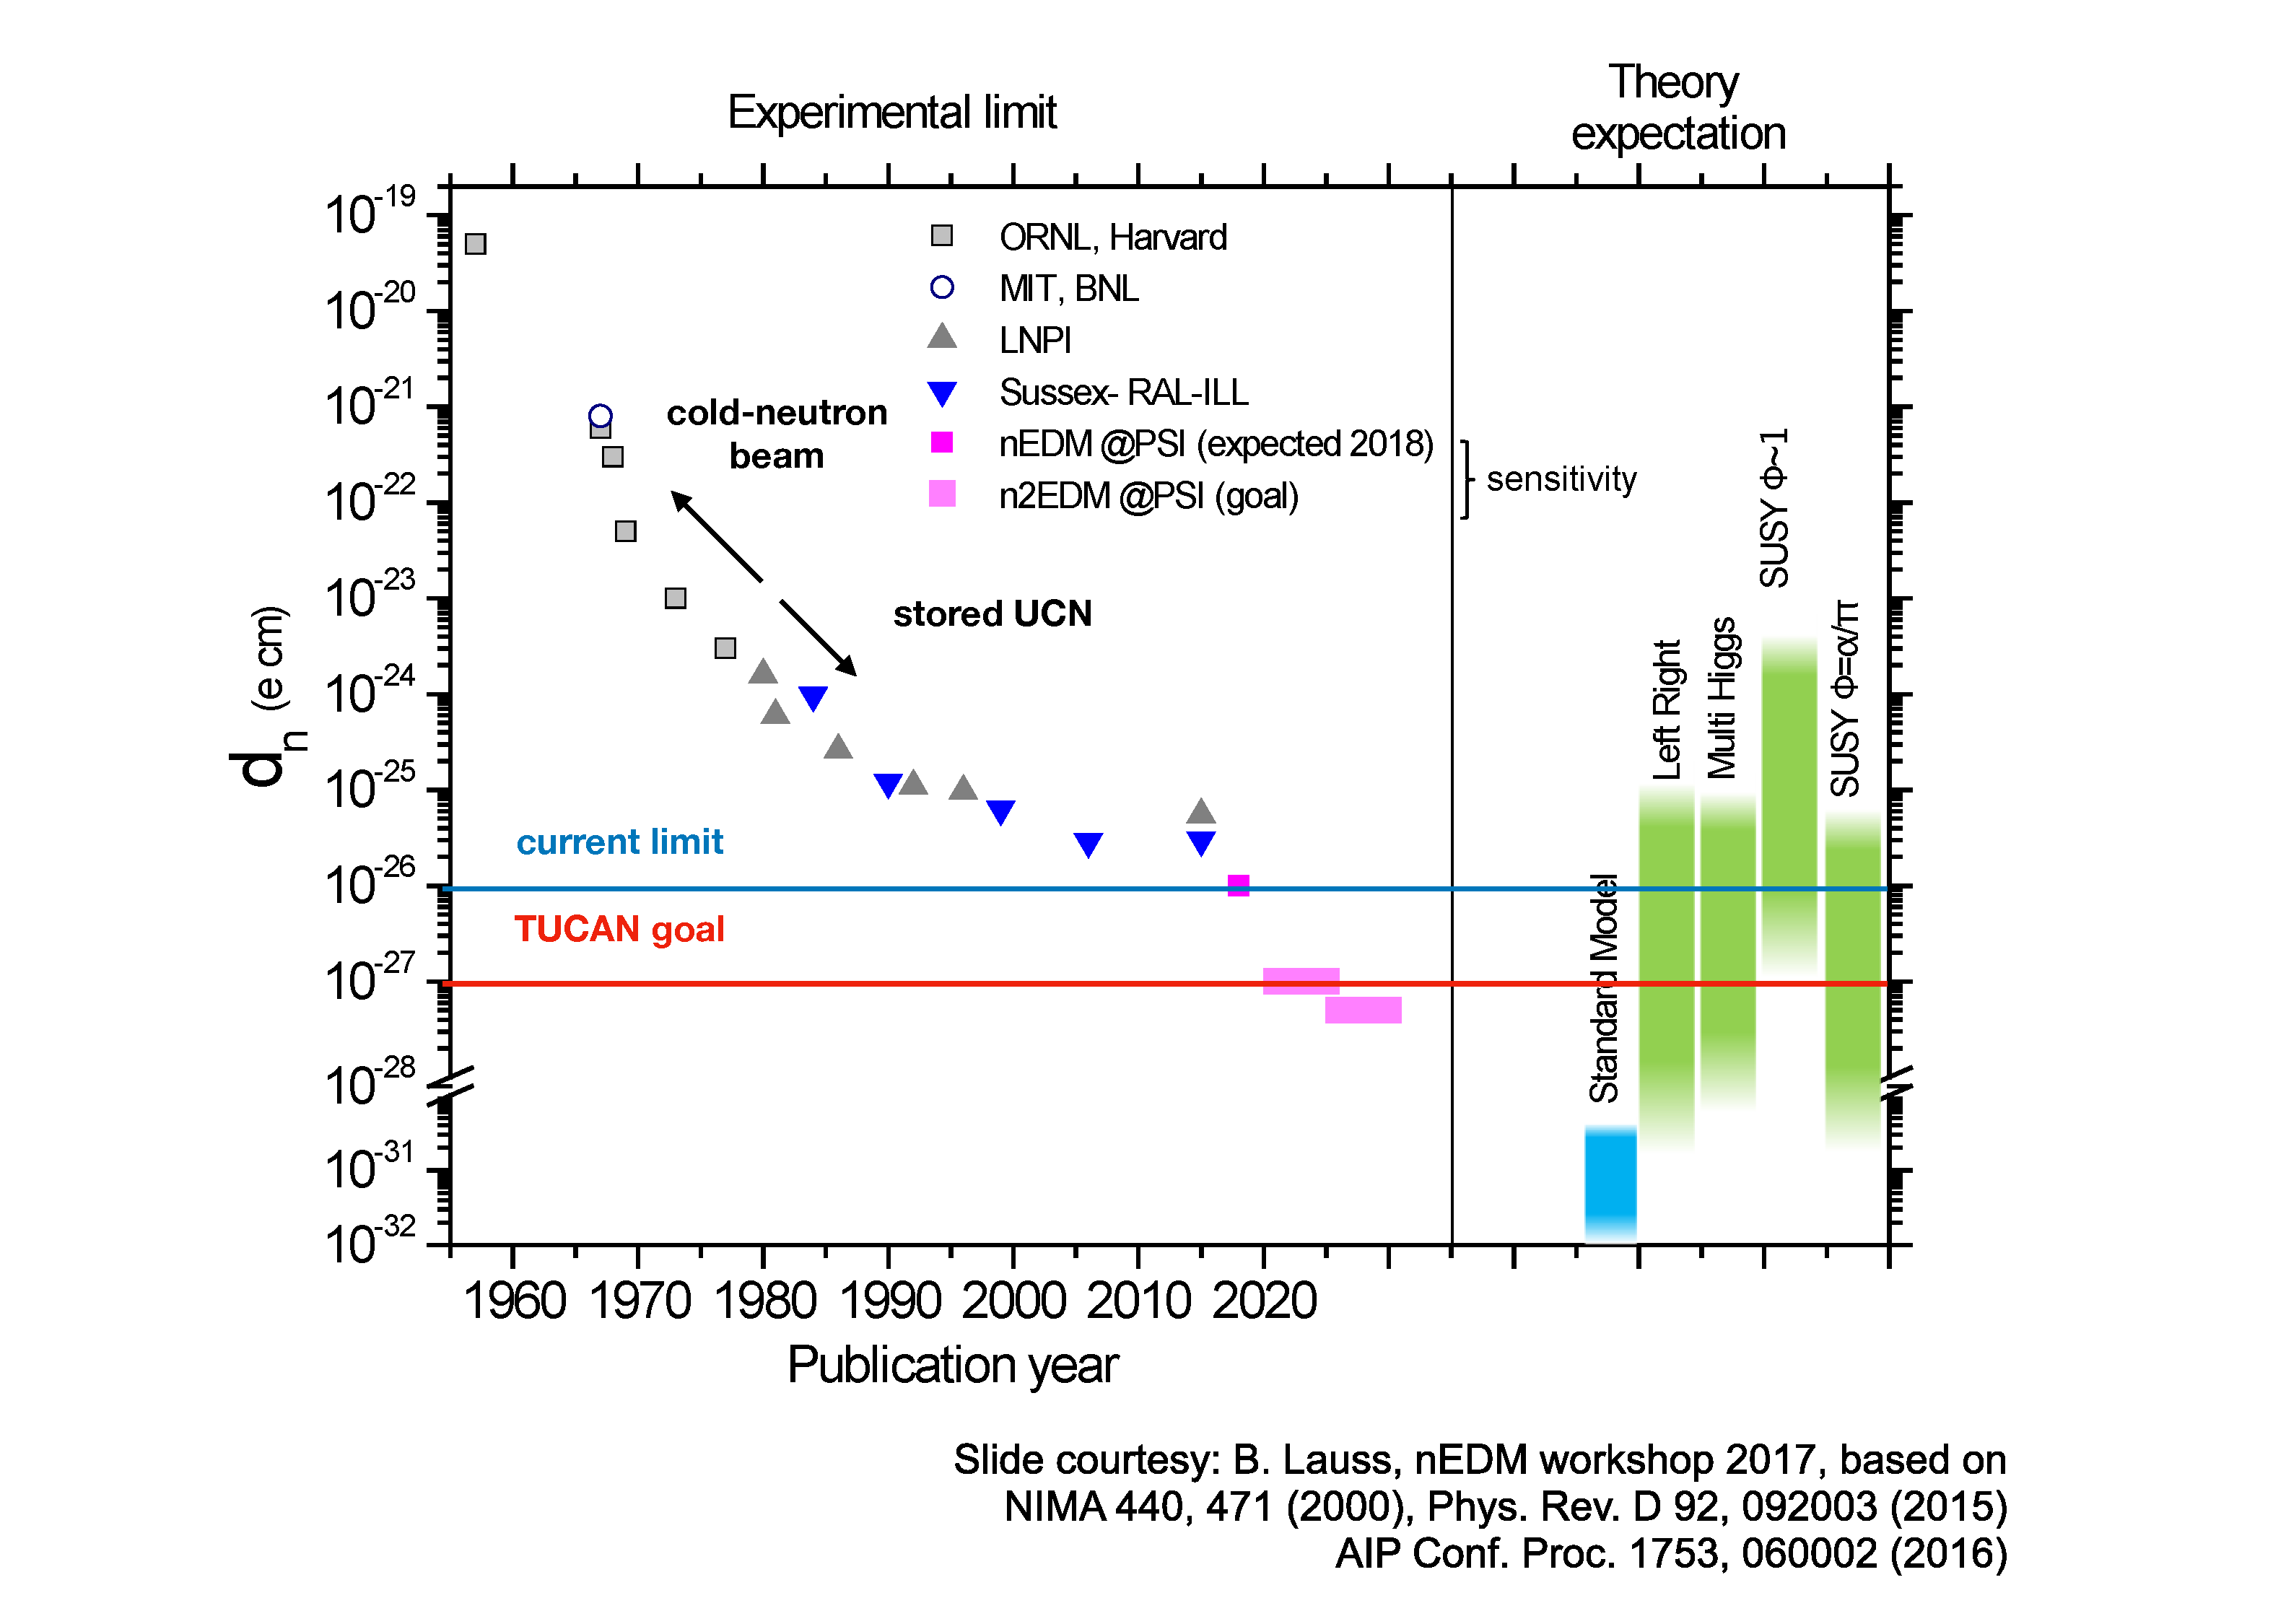
\includegraphics[width=100mm]{history.pdf}
 \caption{Historical development of the experimental upper limit on the nEDM. The method and the location of the experiment are indicated in the legend. The theoretical predictions according to SM and BSM theories are shown on the right.}
\end{figure}

\begin{figure}[tbh]
 \centering
 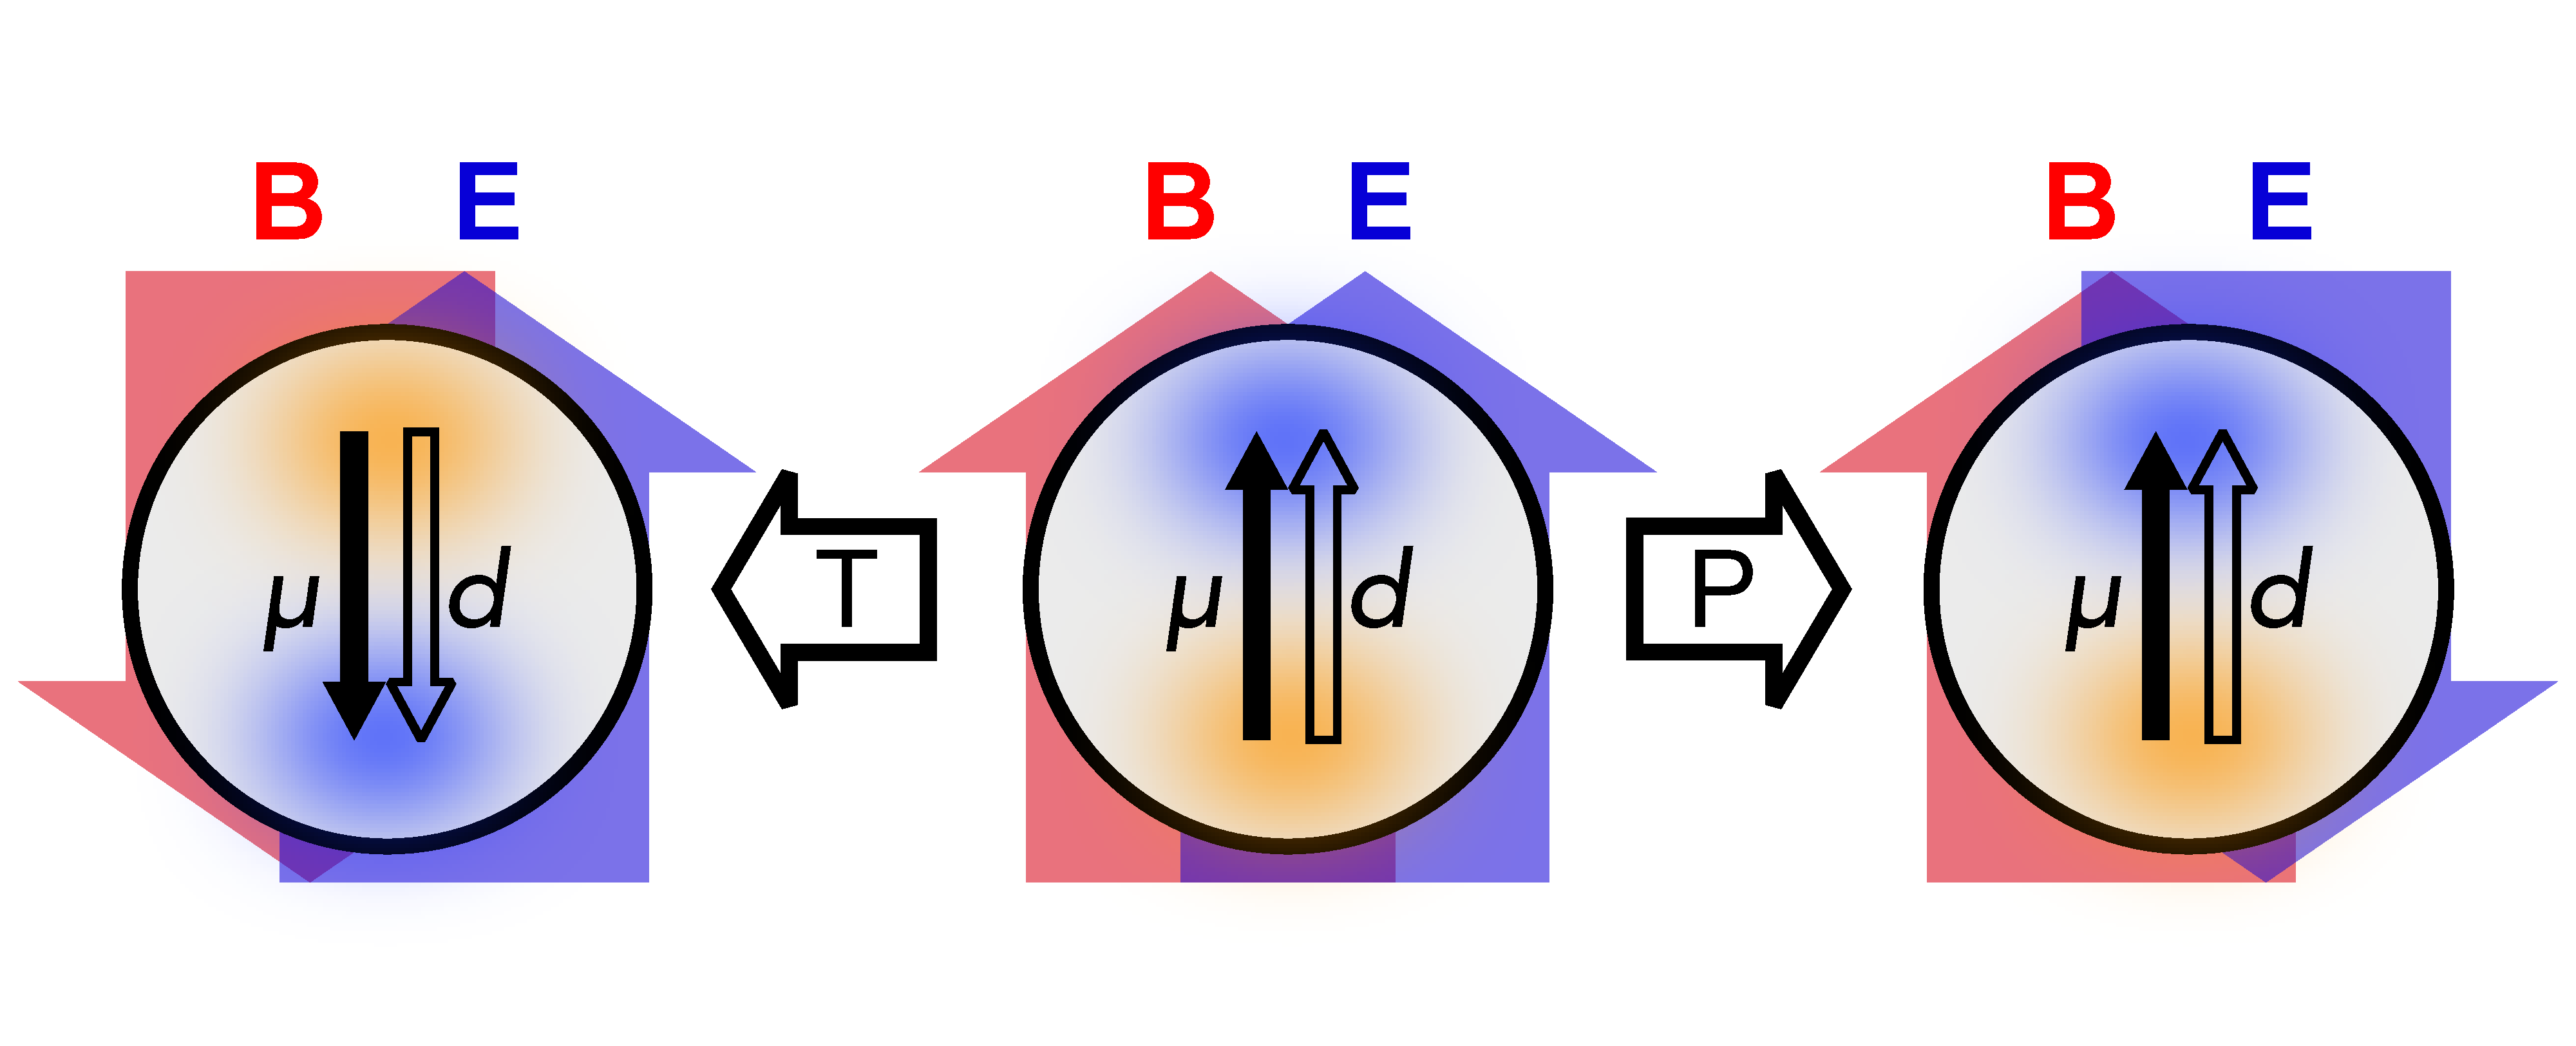
\includegraphics[width=80mm]{nEDM.pdf}
 \caption{スピン偏極解析の原理}
\end{figure}

\end{comment}


%\subsection{Ultra Cold Neutron (UCN)}
\section{nEDM measurement}
\subsection{Principle of nEDM measurement}
中性子は磁気モーメント$\bf \mu_n$を持つため、磁場$\bf \it B$中でラーマー歳差運動を行う。中性子が、EDMを持つと仮定すると、電場$\bf \it E$とも相互作用し位相が変化し、ハミルトニアン$\bf \it H$は次のように記述される。
\begin{equation}
   \bf \it  H =−\mu_n \cdot B−d_n\cdot E
\end{equation}
(fig.1)に示すような、中性子に印加する磁場と電場の向きが平行、反平行の場合の歳差運動の周波数$\hbar \omega_{\uparrow\uparrow},\,\hbar \omega_{\uparrow\downarrow}$は、以下のように書ける。

\begin{equation}
  \hbar \omega_{\uparrow\uparrow} =
  2\mu_n \cdot B+2d_n\cdot E
\end{equation}

\begin{equation}
  \hbar \omega_{\uparrow\downarrow} =
  2\mu_n \cdot B-2d_n\cdot E
\end{equation}

このように、磁場と電場が平行の場合、反平行の場合で中性子の歳差運動の周波数が異なる。よって、周波数を測定し、その差分$\delta \omega=(\omega_{\uparrow\uparrow}-\omega_{\uparrow\downarrow})$を取ることで、EDMの大きさとを得ることができる。

\begin{equation}
    d_n=\frac{\hbar(\omega_{\uparrow\uparrow}-\omega_{\uparrow\downarrow})}{4E}=\frac{\hbar\delta\omega}{4E}
\end{equation}

歳差運動の周波数は、ラムゼー共鳴法\cite{Ramsey}によって測定される。nEDMの大きさの統計感度は、次の式で表される。

\begin{equation}
    \delta d_n=\frac{\hbar}{2\alpha E t_c \sqrt{N}}
\end{equation}

ここで、$\alpha$は中性子の偏極度を表すパラメータ、$t_c$は中性子と電磁場との相互作用時間、Nは中性子の個数を表す。

\begin{figure}[tbh]
 \centering
 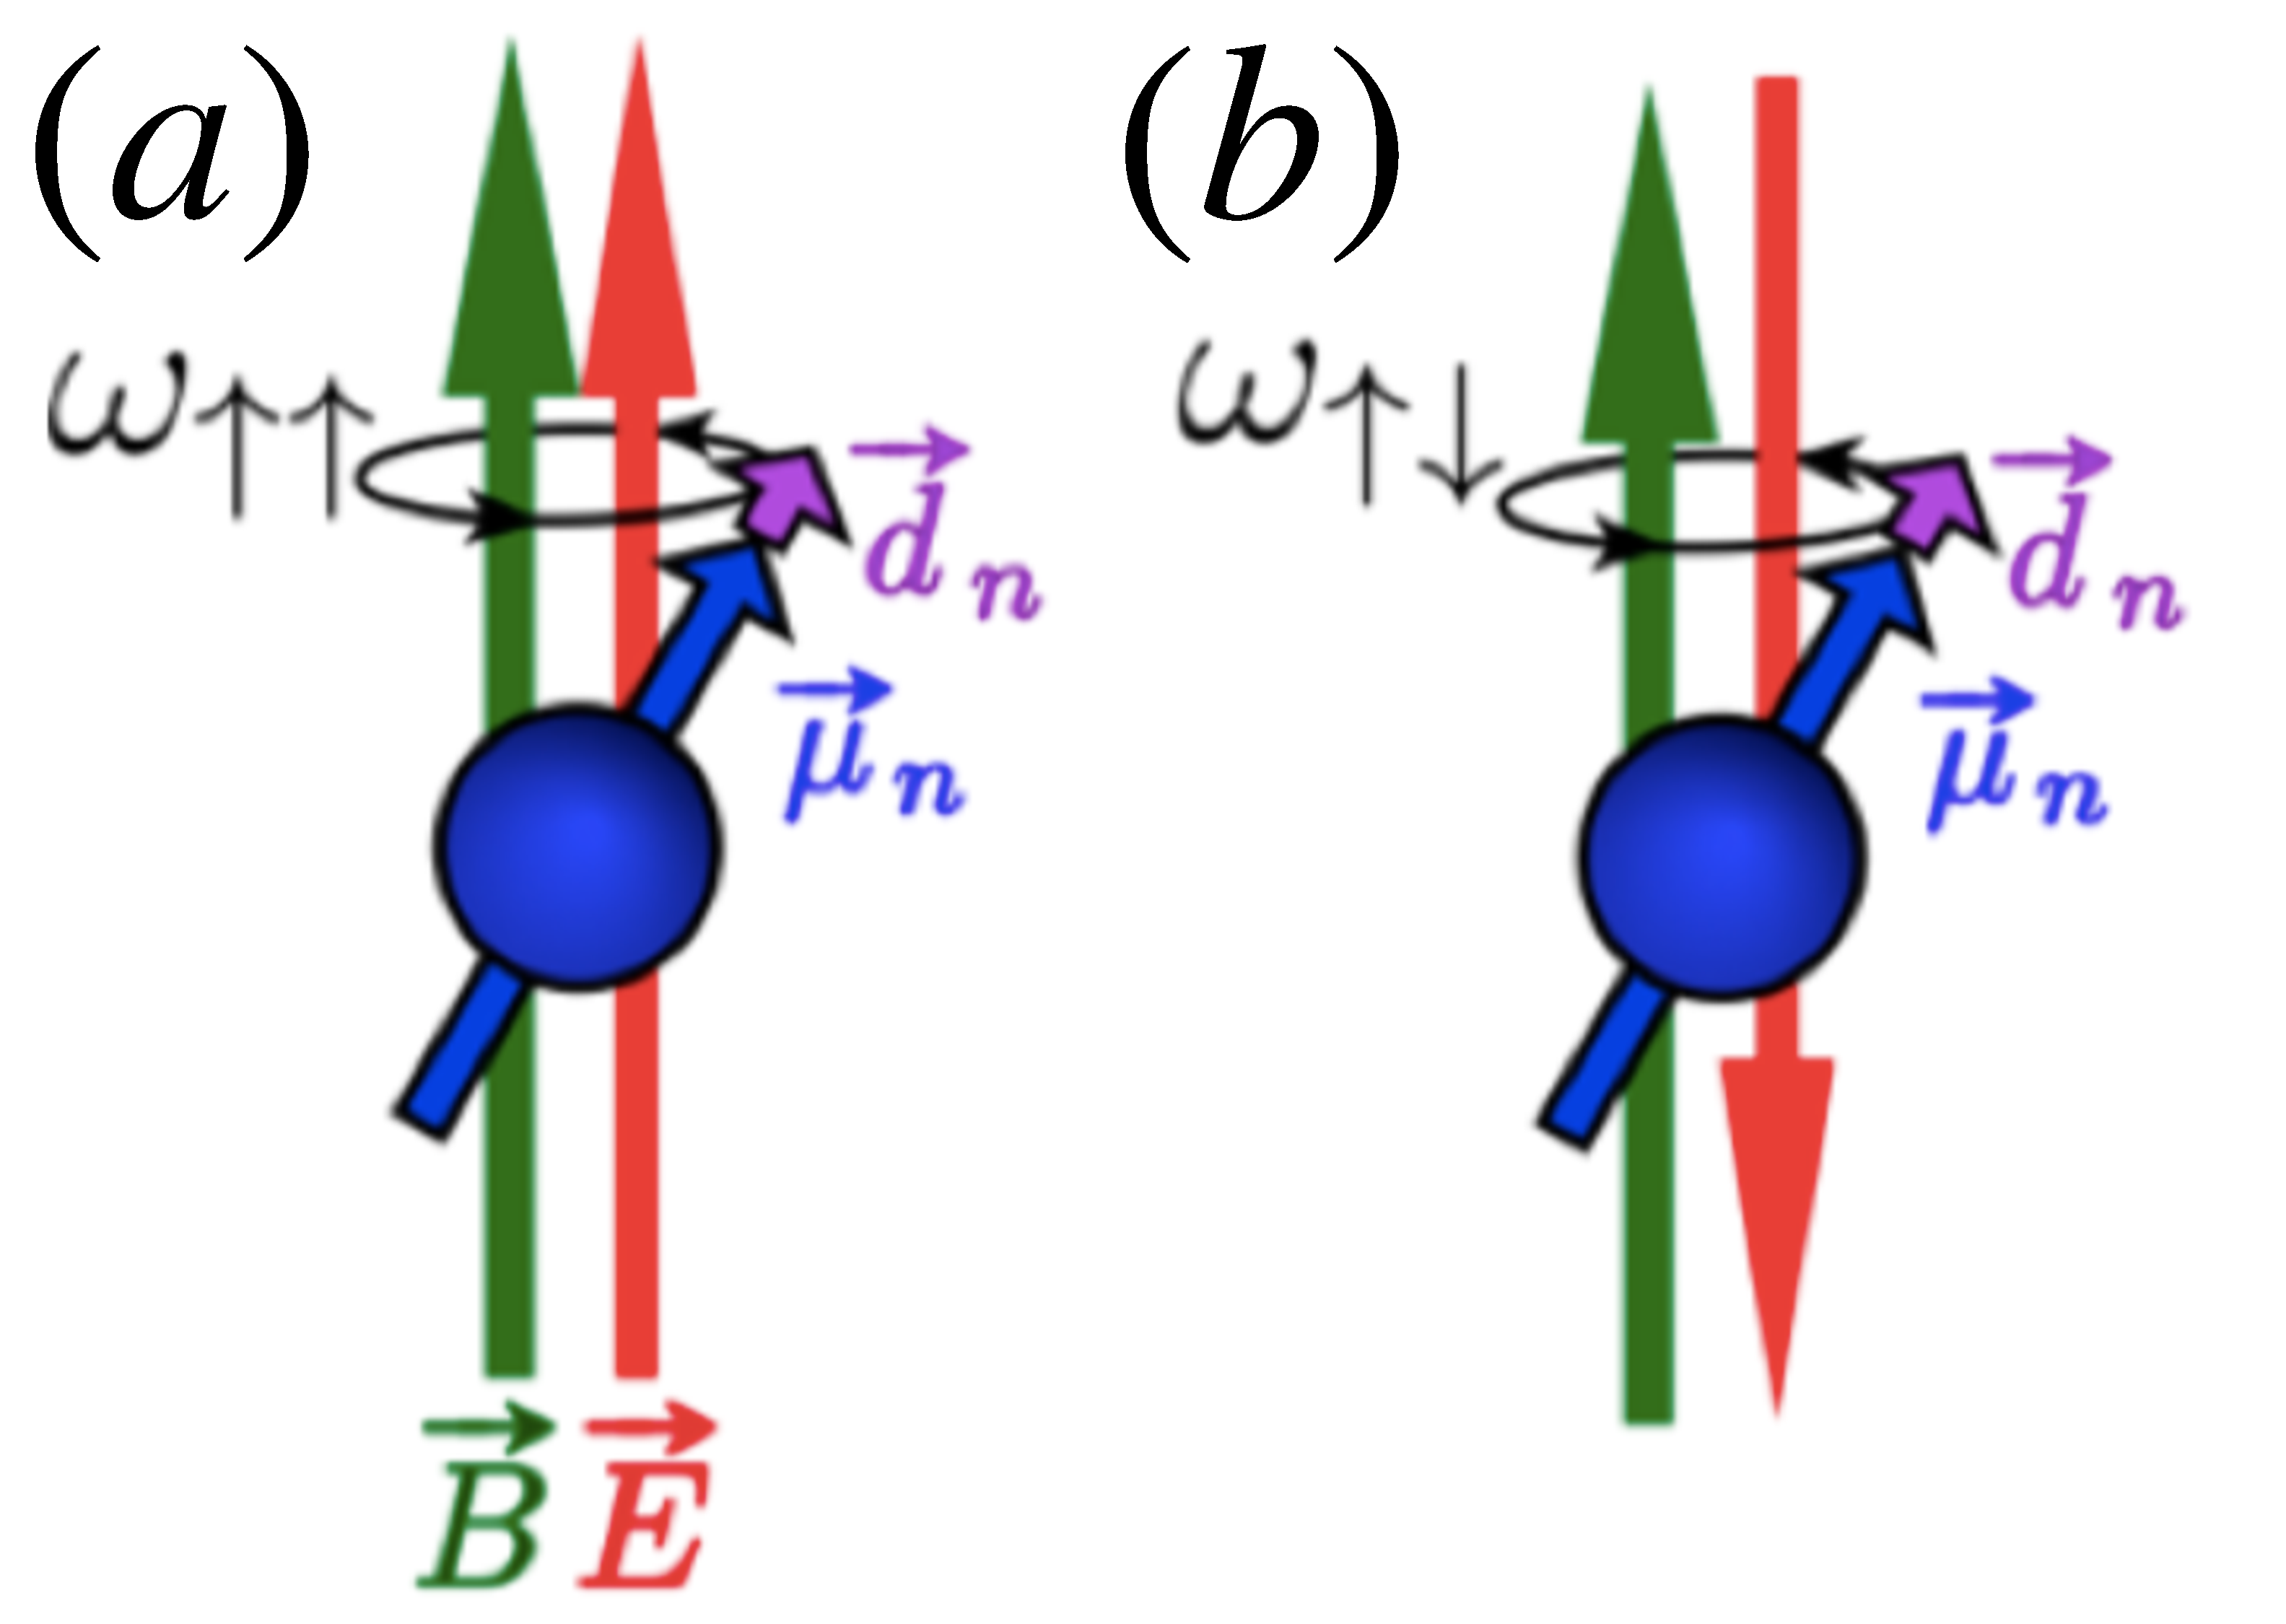
\includegraphics[width=60mm]{EDM_pri.pdf}
 \caption{Precession when the magnetic and electric fields applied to the neutron are parallel (a) and antiparallel (b).}
 %中性子に印加する磁場と電場が平行の場合の歳差運動(a)、反平行の場合の歳差運動(b)}
\end{figure}

%\subsection{Larmor frequency measurement by the Ramsey method}

\subsection{Principle of UCN spin analyzer}
中性子は磁気モーメント$\mu_n$を持つ。磁場$B$中で中性子が感じるポテンシャルは$U_{\rm M}=-\mu_n\cdot {\bf \it B}$と表される。$|\mu_n|=60.3\,\rm neV$であるため、$2\,\rm T$の磁場中でスピンが磁場に対して平行な中性子と反平行な中性子では感じるポテンシャルの差が$\sim 240\,\rm neV$となる。この性質はUCNのspin analyzerに利用されている。我々は、UCNを偏極するために厚さ$\sim 100\,\rm nm$の磁化させた鉄薄膜を用いている。(fig.1 a)のように磁化させた鉄薄膜を通過する際、
中性子が感じるポテンシャルの大きさは、スピンの向きを
$\uparrow, \downarrow$として次のように表される。

\begin{equation}
    V_{\uparrow}=V_{\rm Fe}-\mu_n\cdot {\bf \it B}=209\,\rm neV- 60\,\rm neV/T \cdot {\bf \it B}
\end{equation}

\begin{equation}
    V_{\downarrow}=V_{\rm Fe}+\mu_n\cdot {\bf \it B}=209\,\rm neV+60\,\rm neV/T \cdot {\bf \it B}
\end{equation}

ここで$V_{\rm Fe}=209\,\rm neV$は鉄のフェルミポテンシャルである。




\begin{figure}[tbh]
 \centering
 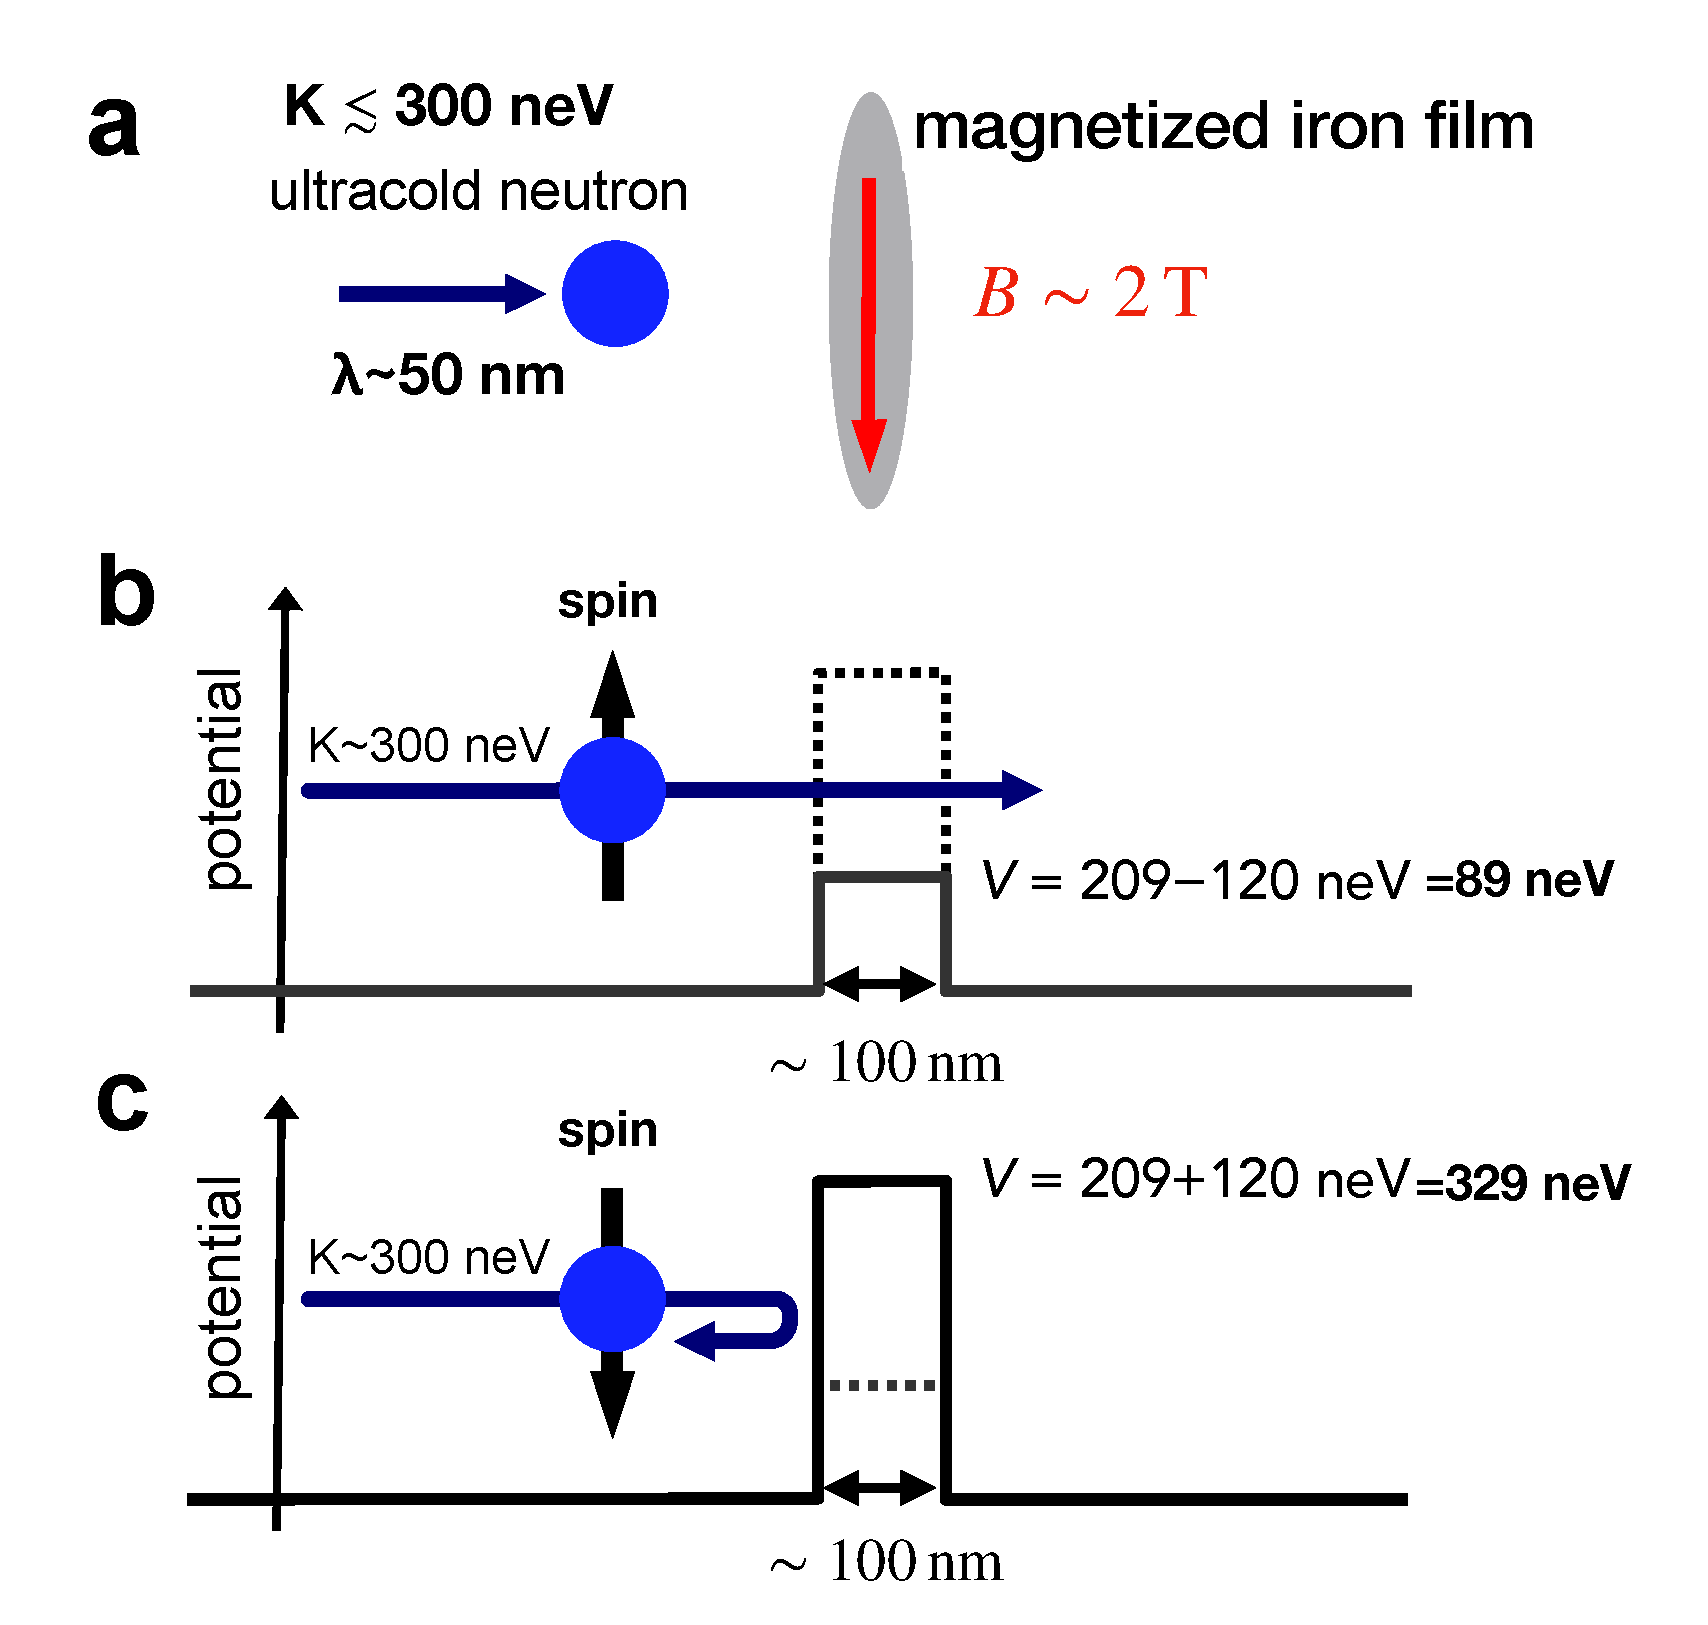
\includegraphics[width=80mm]{potential_spin.pdf}
 \caption{}
\end{figure}



\subsection{The TRIUMF Ultra-Cold Advanced Neutron collaboration}

我々は、TRIUMFの陽子ビームラインにて大強度UCN源の開発を行っている(fig.2)。このビームラインでは、ヘリウムクライオスタットにより、これまでのUCNビーム強度の約40倍である、$40\mu A$の強度を得ることができる。生成したUCNは、超伝導磁石によって偏極され、nEDM spectrometerへ導入される。$\sim 100\,\rm s$間の蓄積の後、Simultaneous Spin Analyzer (SSA)にて偏極度を測定することで、nEDMの探索が可能となる。

\begin{figure}[tbh]
 \centering
 \includegraphics[width=140mm]{overall.pdf}
 \caption{ Overview of the new UCN source and the nEDM spectrometer of the TUCAN collaboration. Spallation neutrons from the tungsten target are moderated to cold neutron energies and then converted to UCNs in the production volume filled with He-II. The UCNs are polarized by a 3.5 T magnetic field of the superconducting magnet and led into the nEDM spectrometer through UCN guides.The red waxy area is the Simultaneous Spin Analyzer (SSA). An enlarged version of this is shown in (fig.4).}
\end{figure}


\subsection{Simultaneous Spin Analyzer (SSA)}
cell内で$\sim 100\,\rm s$の間、電場を印加し続けたUCNに対してSimultaneous Spin Analyzer (SSA)を用いて偏極解析を行う。SSAの概略図は(fig.3)に示す。永久磁石によって磁化した鉄薄膜を用いて特定の向きのスピンの中性子のみを通過させ、検出する。左右2つのアームで、それぞれ異なるスピンの中性子を同時に測定することができる。また、spin flipperのON, OFFを切り替えることで、左右の検出器を入れ替えて測定を行うことができ、系統的な誤差を減らすことができる。我々は今回、SSA内のiron filmの開発を行った。


\begin{figure}[tbh]
 \centering
 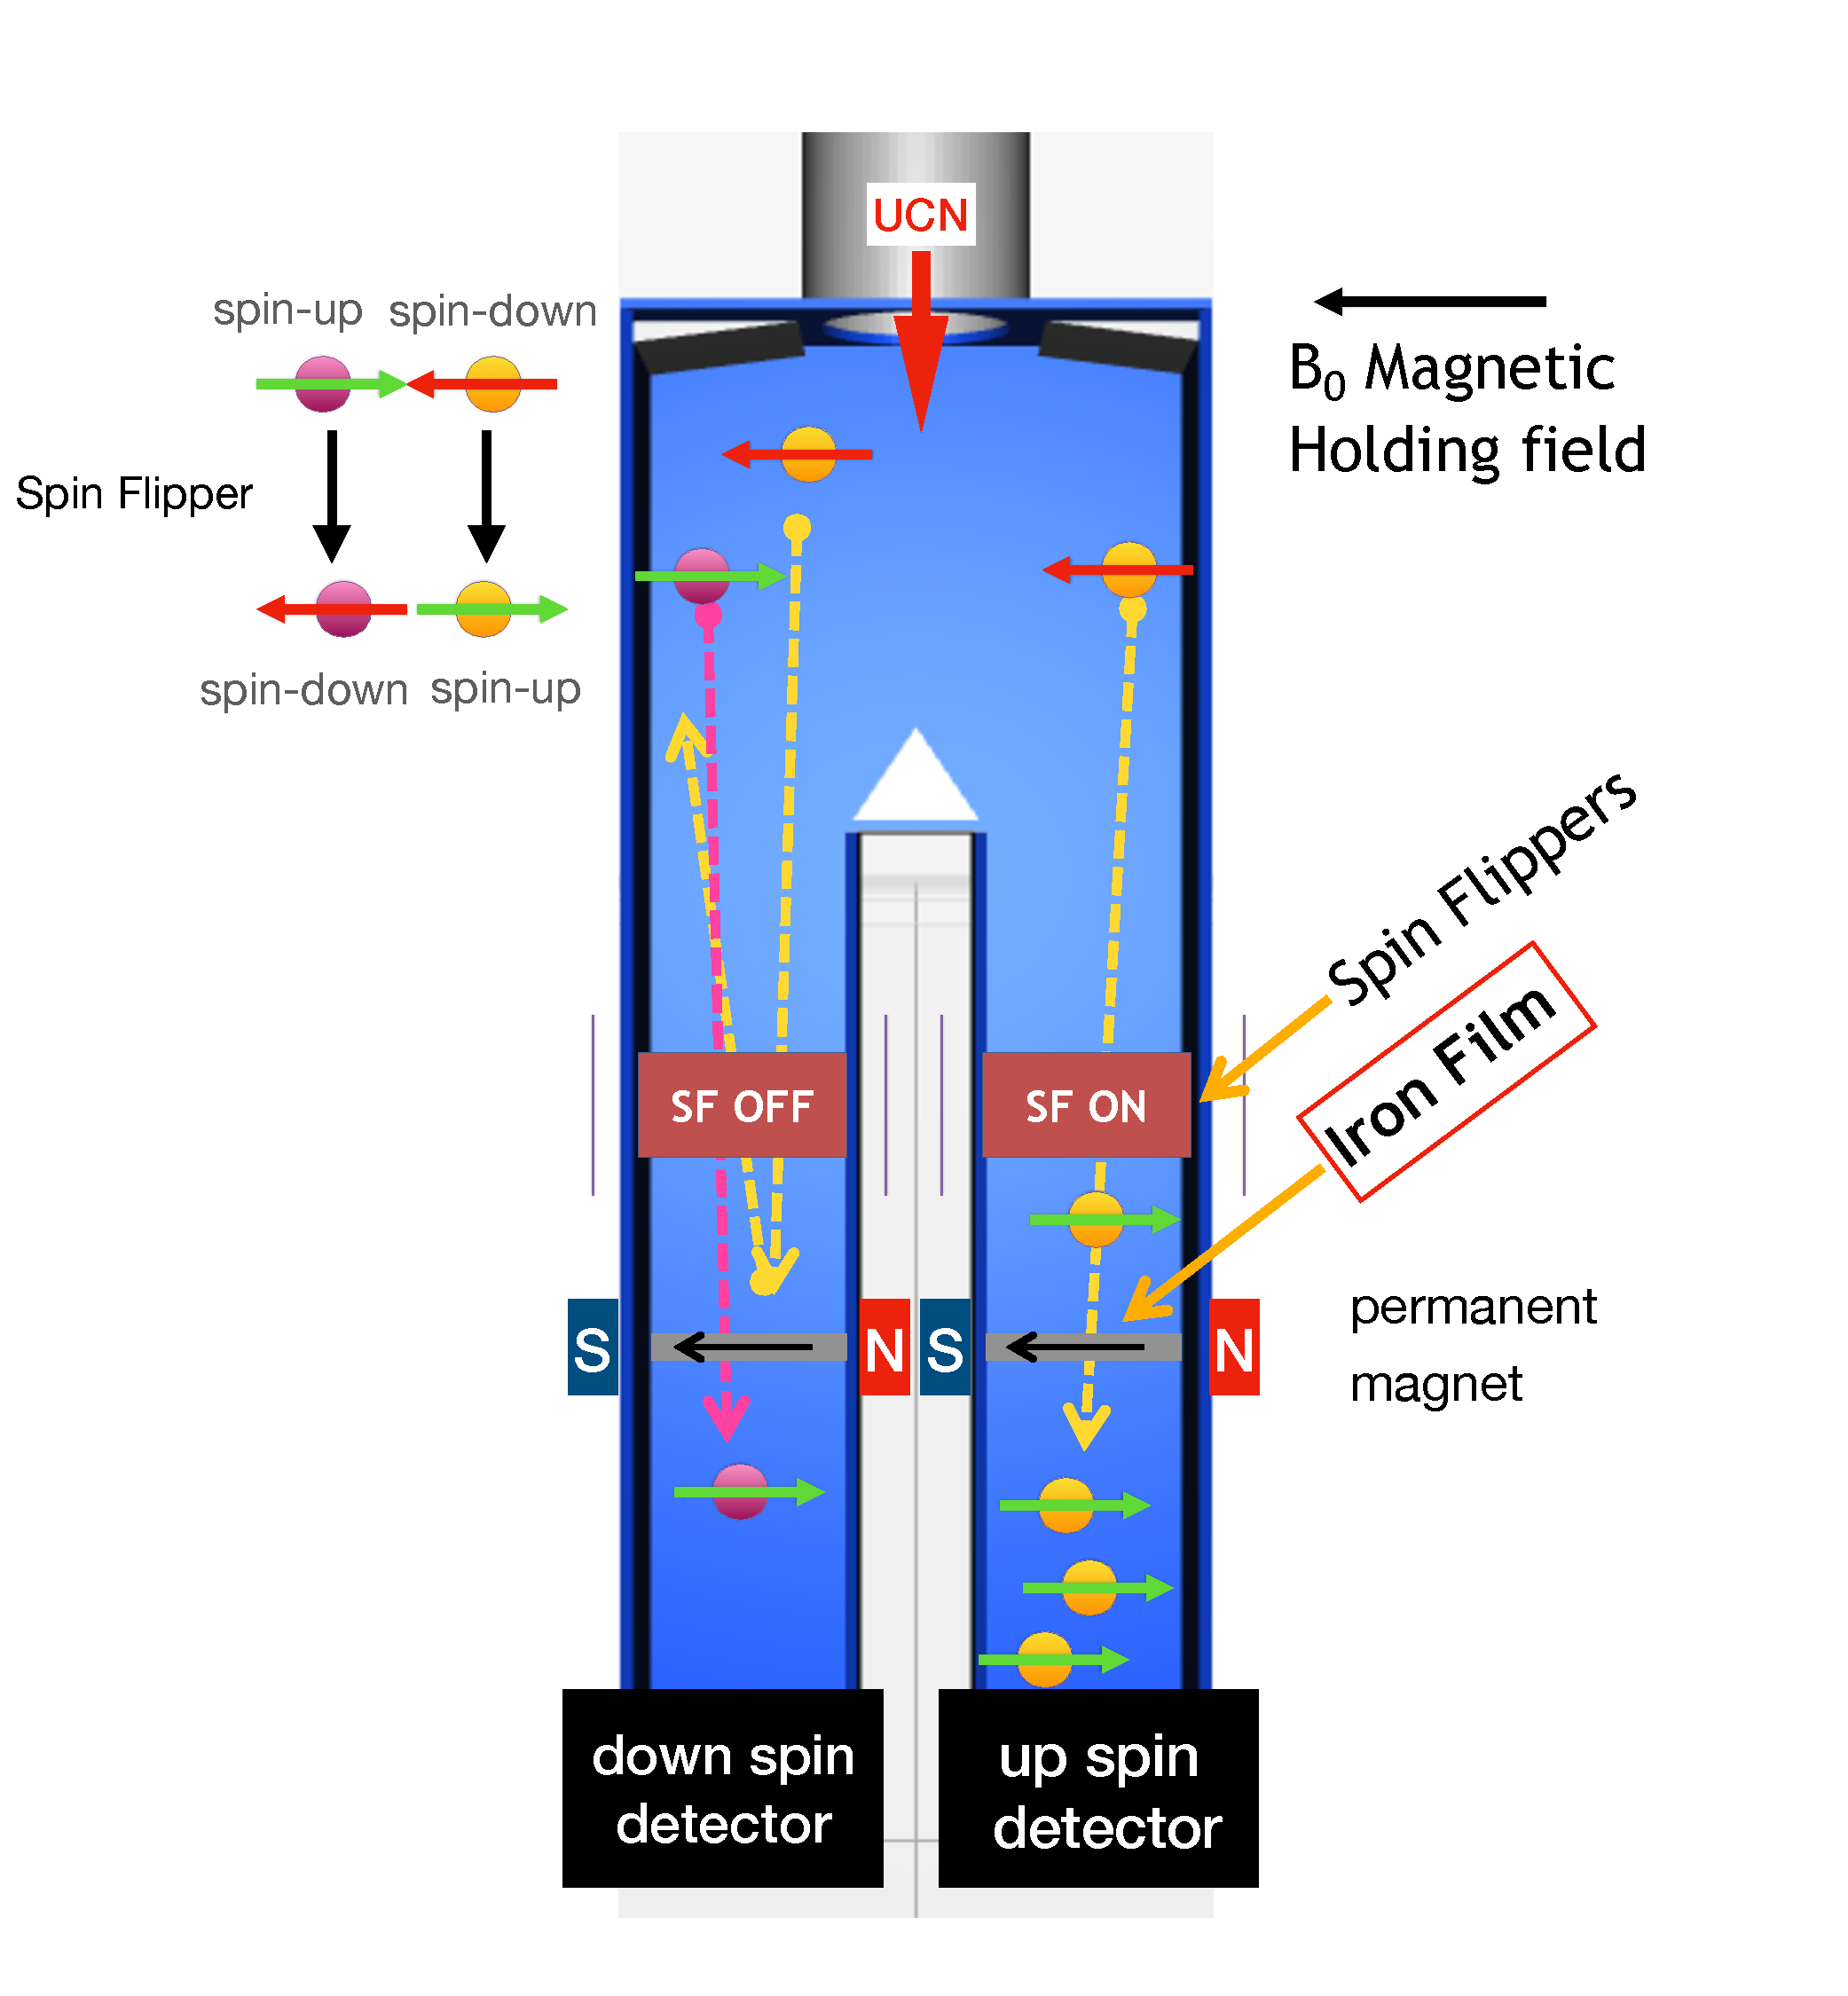
\includegraphics[width=70mm]{SSA_1.pdf}
 \caption{Overview of Simultaneous Spin Analyzer (SSA).UCNs with spin orientations parallel to the direction of the magnetic field in the iron film (red) and UCNs with spin orientations antiparallel to the magnetic field (green) are inserted from the top.The spins can be flipped by the spin flipper, and only the spins in the desired orientation can be transmitted and detected.}
\end{figure}

\section{Development and Evaluation of UCN polarization analyzer films at KURNS}
\subsection{Development of UCN polarization analysis film}

Institute for Integrated Radiation and Nuclear Science, Kyoto University(KURNS)の、ion beam sputtering system (IBS)を用いて、偏極解析膜を作成した。\cite{Hino}偏極解析膜は、鉄薄膜と基板の2層構造からなる。我々は、鉄薄膜の厚さが約30,60,90 $\rm nm $となる試料を作成した。基板にはシリコン(厚さ 380 $\rm \mu m $)または、アルミニウム(厚さ 25 $\rm \mu m $)を用いた。

\begin{figure}[tbh]
 \centering
 \begin{minipage}{0.3\columnwidth}
  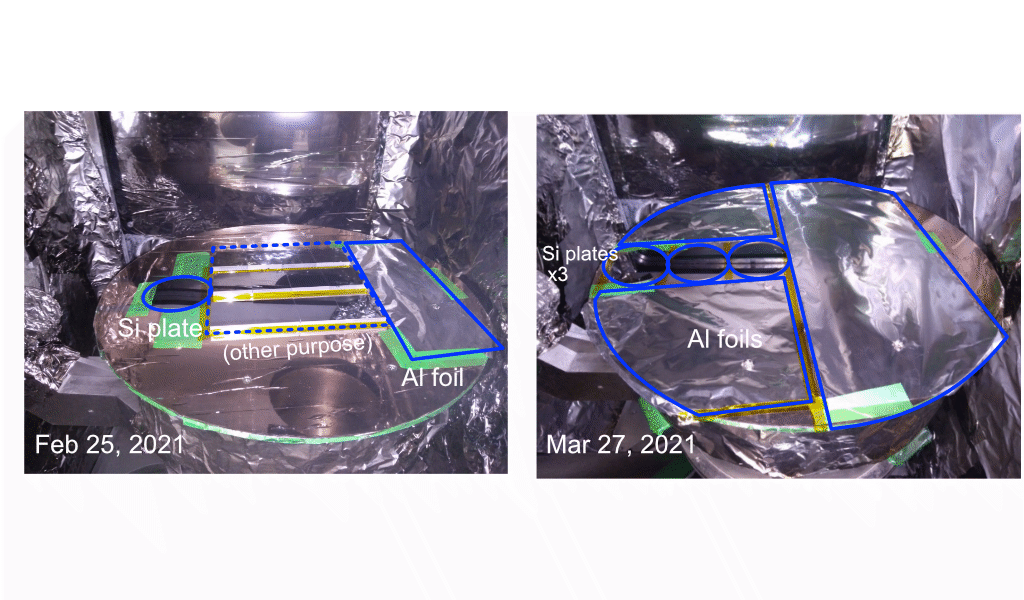
\includegraphics[width=60mm]{KURRI_IBS_samples.png}
  \caption{イオンビームスパッタリング装置を用いた試料作成の様子}
 \end{minipage}
 \centering
 \hspace{0.15\columnwidth}
 \begin{minipage}{0.3\columnwidth}
  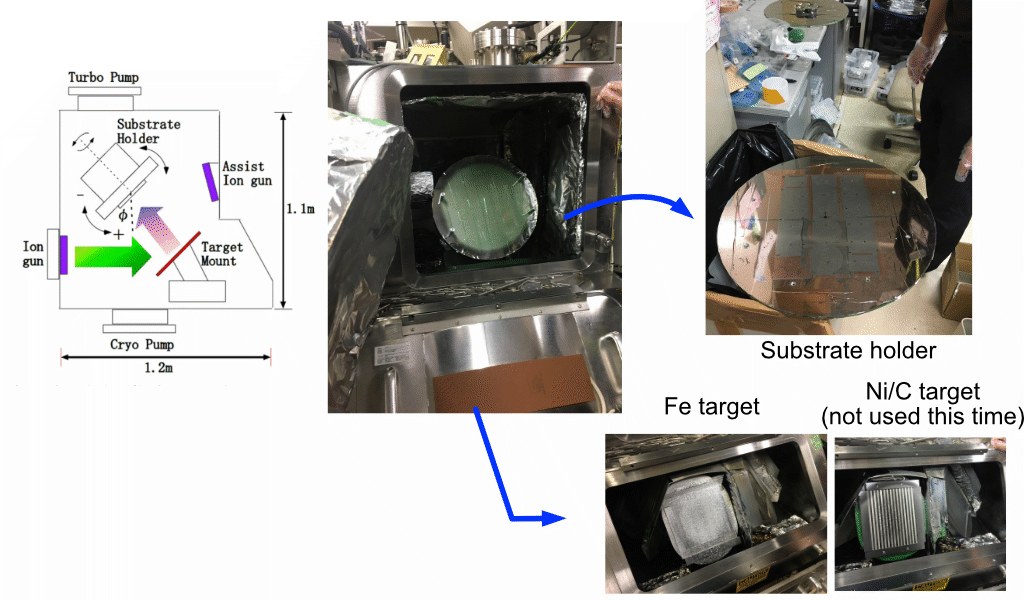
\includegraphics[width=70mm]{KURRI_IBS_Ni.png}
  \caption{イオンビームスパッタリング装置の概要}
 \end{minipage}
 \figlab{sample}
\end{figure}

\subsection{Hysteresis curve measurement}
%\subsection{Evaluation of UCN polarization analyzer films}
作成した試料のヒステリシス曲線を測定するため、VSM (vibrating sample magnetometer)測定を行なった。(fig,)測定結果から、Si+Feの試料は$5\,\rm mT$以下
で、Al+Feの試料は約$15\,\rm mT$以下で完全に磁化することが確認できた。よって他の測定機器に影響を与えない程度の十分に小さい磁場で十分に磁化することがわかった。

\begin{figure}[tbh]
 \centering
 \begin{minipage}{0.2\columnwidth}
  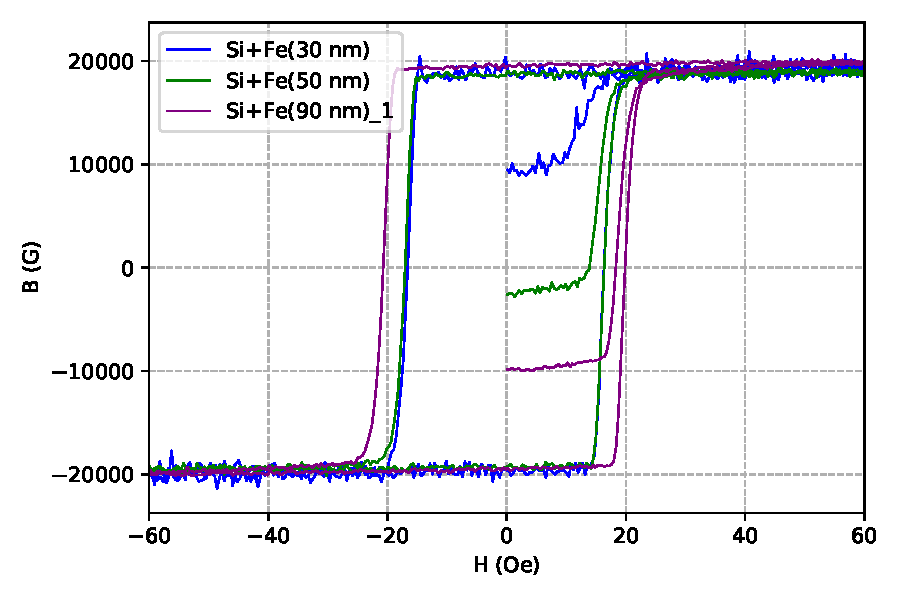
\includegraphics[width=60mm]{summary_Si_JPS_scaled.pdf}
  \caption{Fe+Si基板のBHカーブ。鉄薄膜の厚さによって色を変えている。30 nm (blue), 50 nm (green), 90 nm (purple)}
 \end{minipage}
 \hspace{0.15\columnwidth}
 \centering
 \begin{minipage}{0.2\columnwidth}
  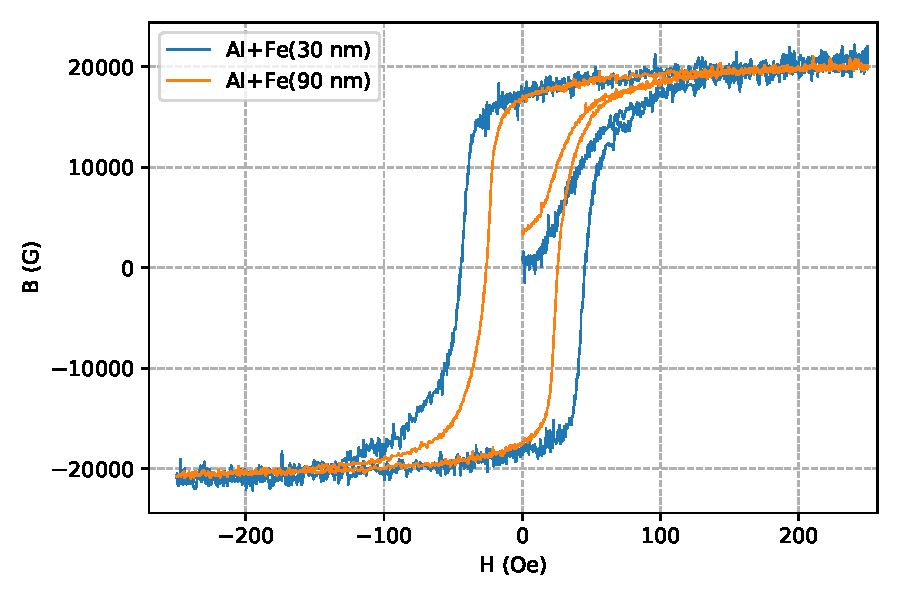
\includegraphics[width=60mm]{Al_summary_JPS_scaled.pdf}
  \caption{Fe+Al基板のBHカーブ。鉄薄膜の厚さによって色を変えている。30 nm (light blue)、90 nm(orange)}
 \end{minipage}
 \figlab{sample}
\end{figure}

\section{Development and Evaluation of UCN polarization analyzer films at J-PARC /MLF}
%\subsection{Neutron reflectometry}
\subsection{Reflectivity measurement of the sample}
2021年7月に、試料のフェルミポテンシャルの大きさを測定するため、J-PARKのMaterials and Life Science Facility(MLF) BL05 にて、冷中性子 (kinetic
 energies of $\sim 1 \,\rm meV$)を用いた反射率測定を行なった。パルス中性子源の白色中性子線を飛行時間法で検出し,wave length または q に変換することで反射率データを得た。
 
 %白色の冷中性子を用いて、試料の反射率を測定すると、ある波長を境に反射率が急激に増加するため、
\subsubsection{Beam polarization measurement}

中性子ビームの偏極ミラーによる偏極度を測定した。全体のセットアップを(fig)に示した。横$0.1\,\rm mm$、縦$10\,\rm mm$の中性子ビームを$8.3\,\rm mrad$の入射角で偏極ミラーに入射し、下流 の RPMT で反射波と透過波の両方を検出した。
\begin{figure}[tbh]
 \centering
 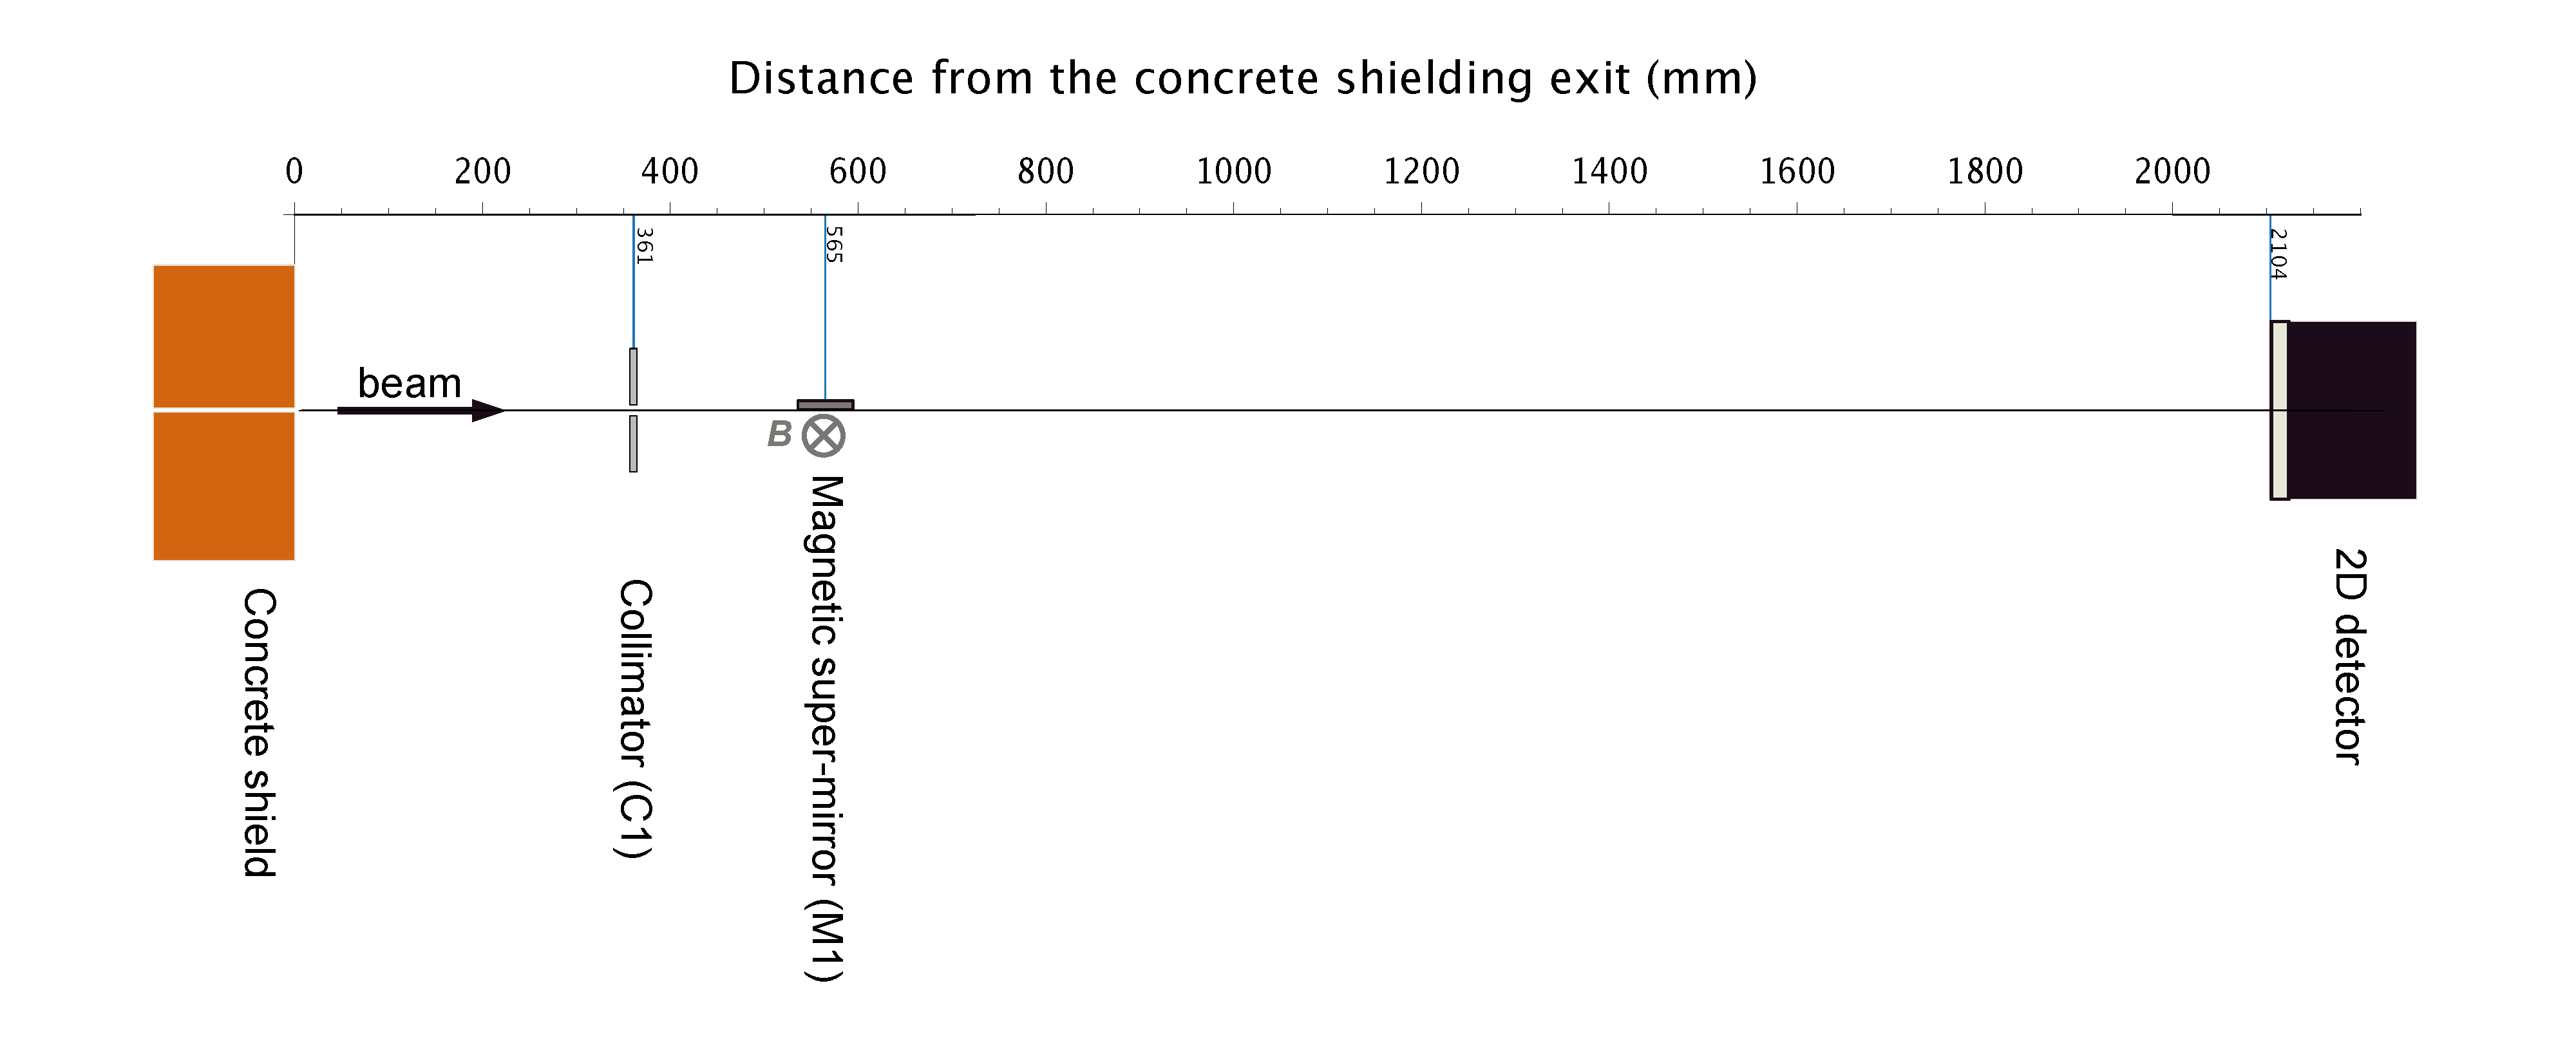
\includegraphics[width=130mm]{BL05_1.pdf}
 \caption{Setup for polarization measurement of magnetic super mirror}
\end{figure}
反射波と透過波の強度を足し合わせたものを、入射強度
とした。反射率=反射強度/入射強度と定義し、偏極ミラーによる冷中性子の反射率を測定した。(fig,11)

\begin{figure}[tbh]
 \centering
 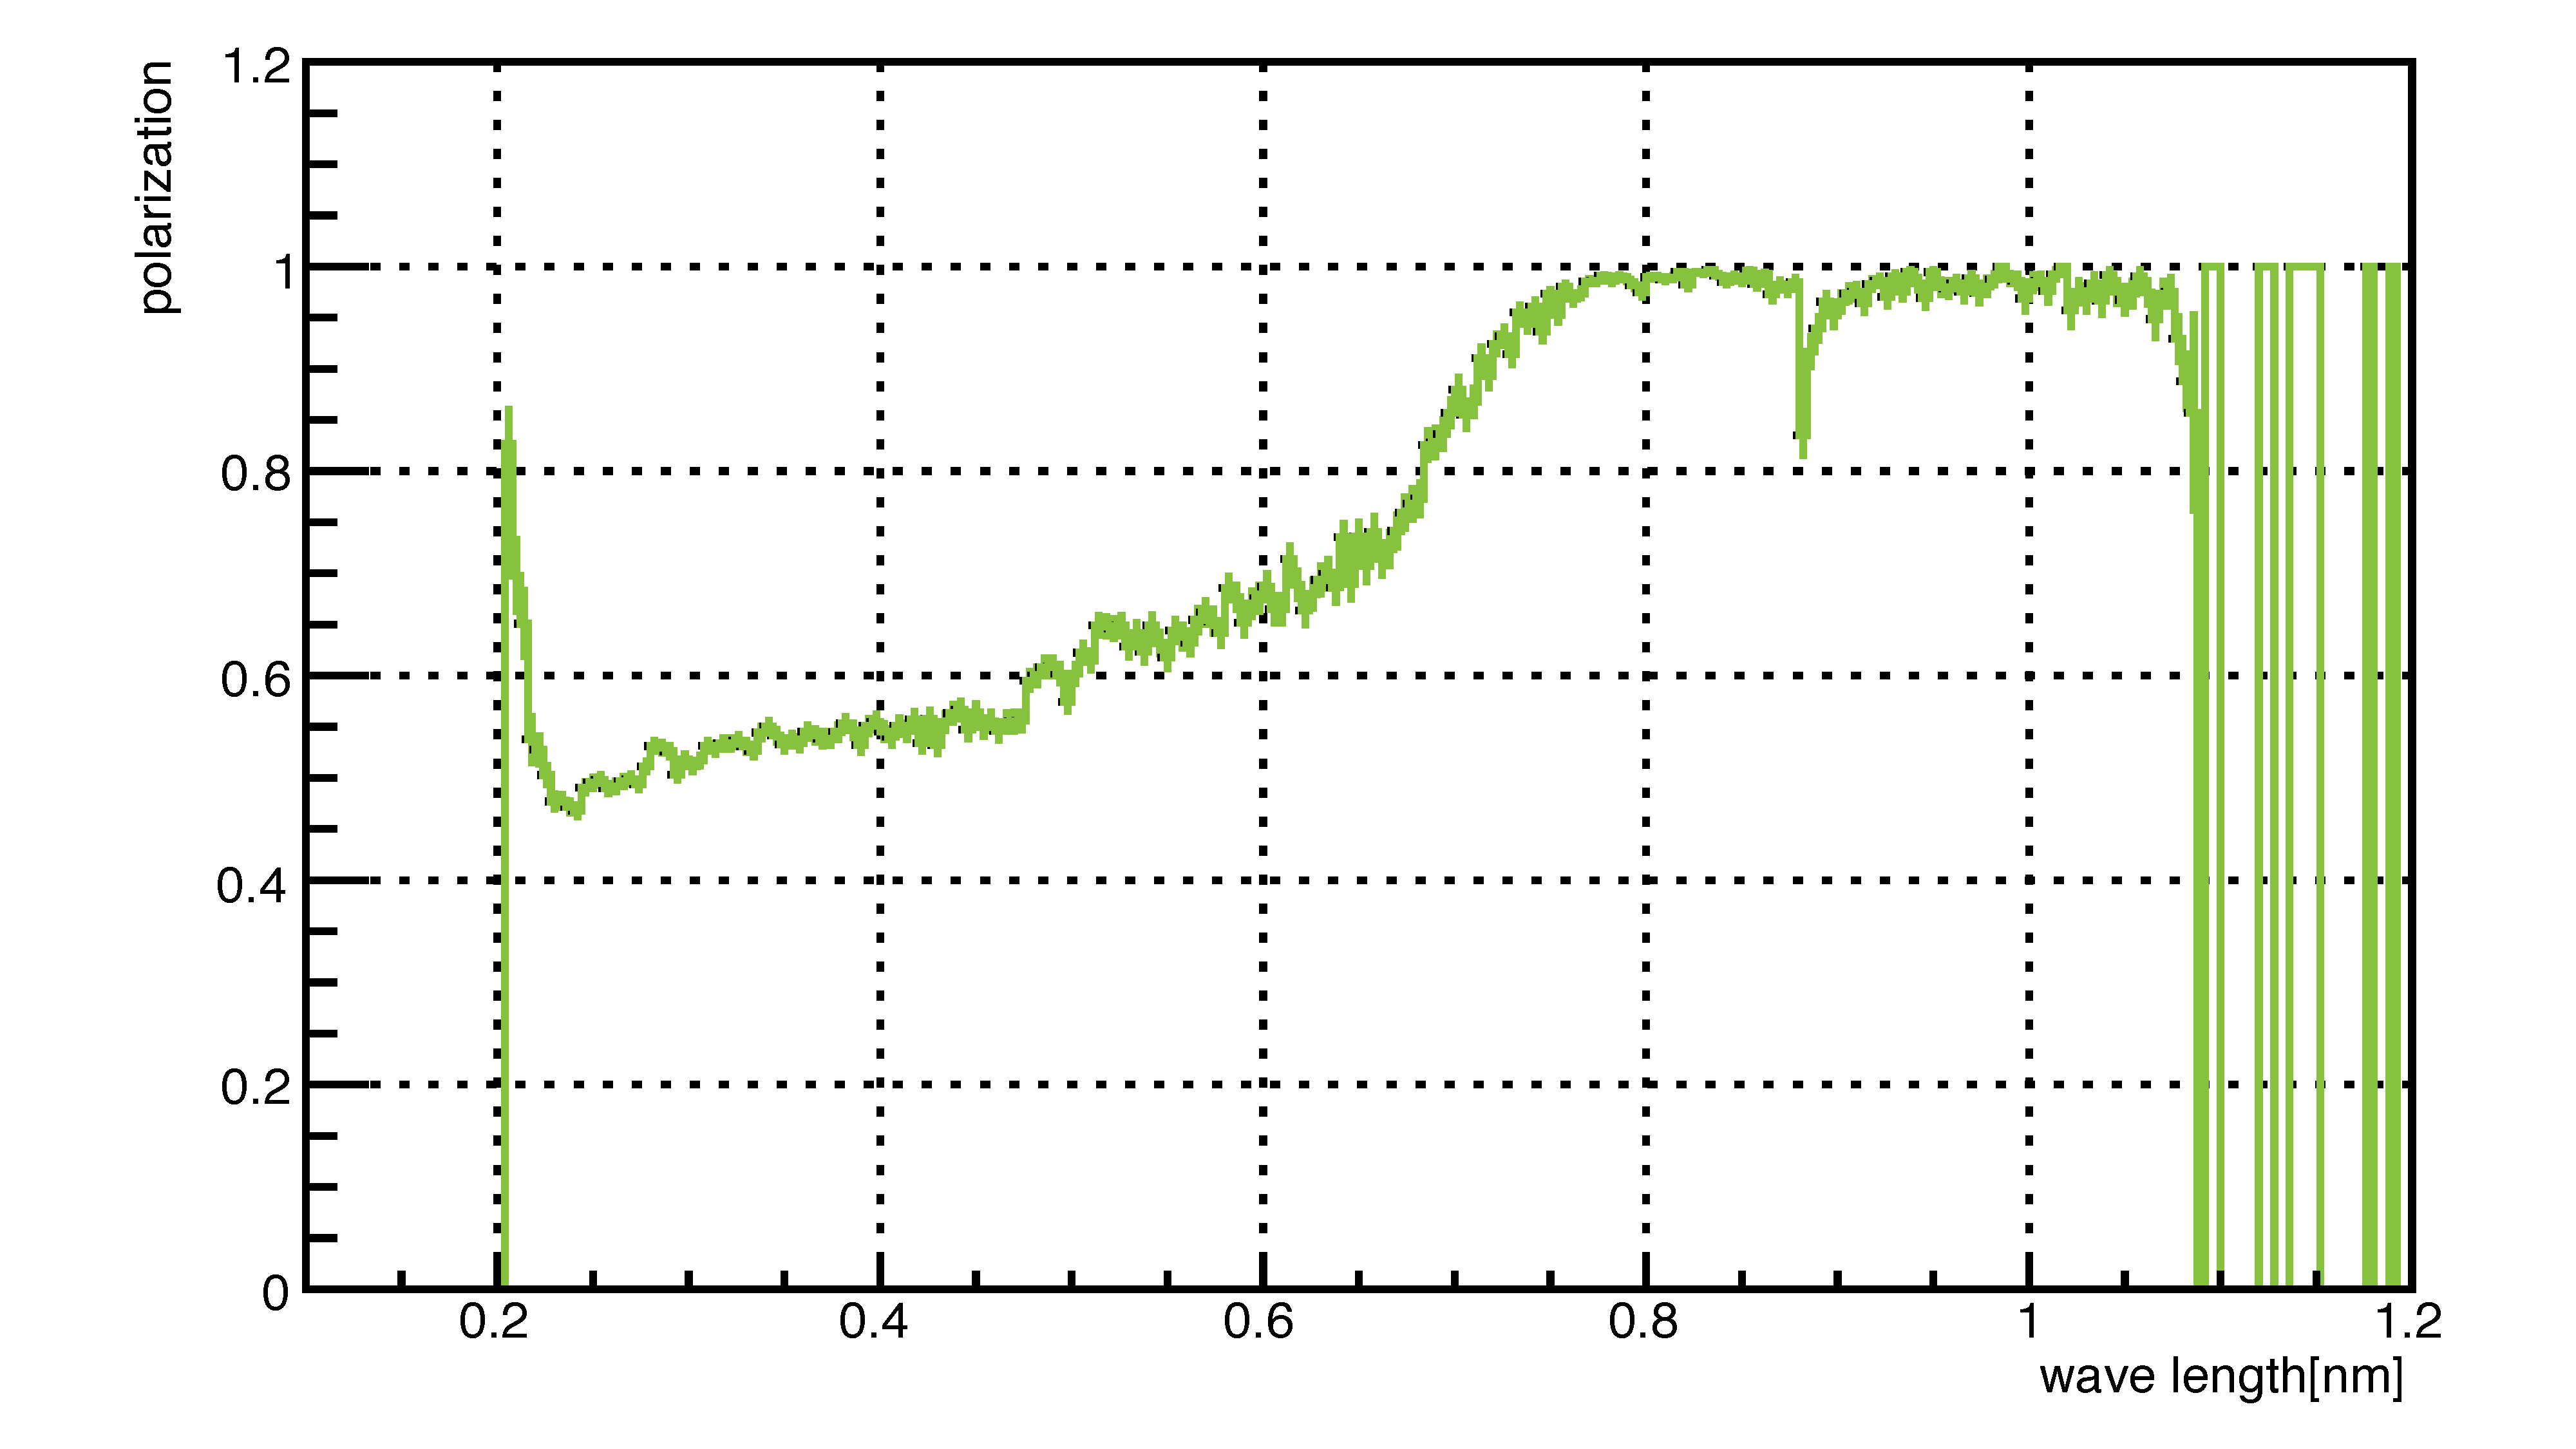
\includegraphics[width=80mm]{polarization.pdf}
 \caption{Wavelength dependence of the reflectivity of the magnetic super mirror}
\end{figure}

\subsubsection{Modeling the polarization of an incident beam}

(fig,11)のとき、偏極ミラーへの入射中性子ビームは偏極されていない。つまり、spin up, spin down
が$50\%$ずつ含まれている。よって、偏極ミラーの反射率$R_{\rm M}$は、spin up の中性子による反射率$R_{\rm up}$、spin down の中性子による反射率$R_{\rm down}$を用いて、次のような式で表すことができる。

\begin{equation}
\label{RM1}
R_{\rm M}=\frac{1}{2} R_{\rm up}+\frac{1}{2} R_{\rm down}
\end{equation}

\begin{equation}
\label{RM2}
R_{\rm up}=\frac{1}{2}R_0\{1.-\tanh((x-m_1 q_c)/W)\}(1.-\alpha(x-q_c))
\end{equation}

$x=4\pi \sin \theta/\lambda$ $m_1$は、偏極ミラーのm値、
それぞれ $R_0=0.99$は全反射領域での反射率、$\alpha$ は臨界反射角でのカットオフまでの傾 き、$W=0.0025$ はカットオフ幅、$m=5.2$ は臨界反射角を表すパラメータである。$q_c$ は $\rm Ni$ の全反射臨界角 $q_c = 0.217 \,\rm nm^-1$である。(参照 横橋修論)\\
$R_{\rm down}$は、(fig,11)の反射率に対して、spline法を用いて関数の形を推定した。$R_{\rm down}$は、偏極ミラーで反射した中性子ビームに含まれるspin upの割合と捉えることもできる。そのため、推定した$R_{\rm down}$のspline関数を用いて、ミラーで反射した中性子の偏極度が決まる。(fig,13)


%(\ref{RM1}), (\ref{RM2})式を

\begin{equation}
\end{equation}

\begin{figure}[tbh]
 \centering
 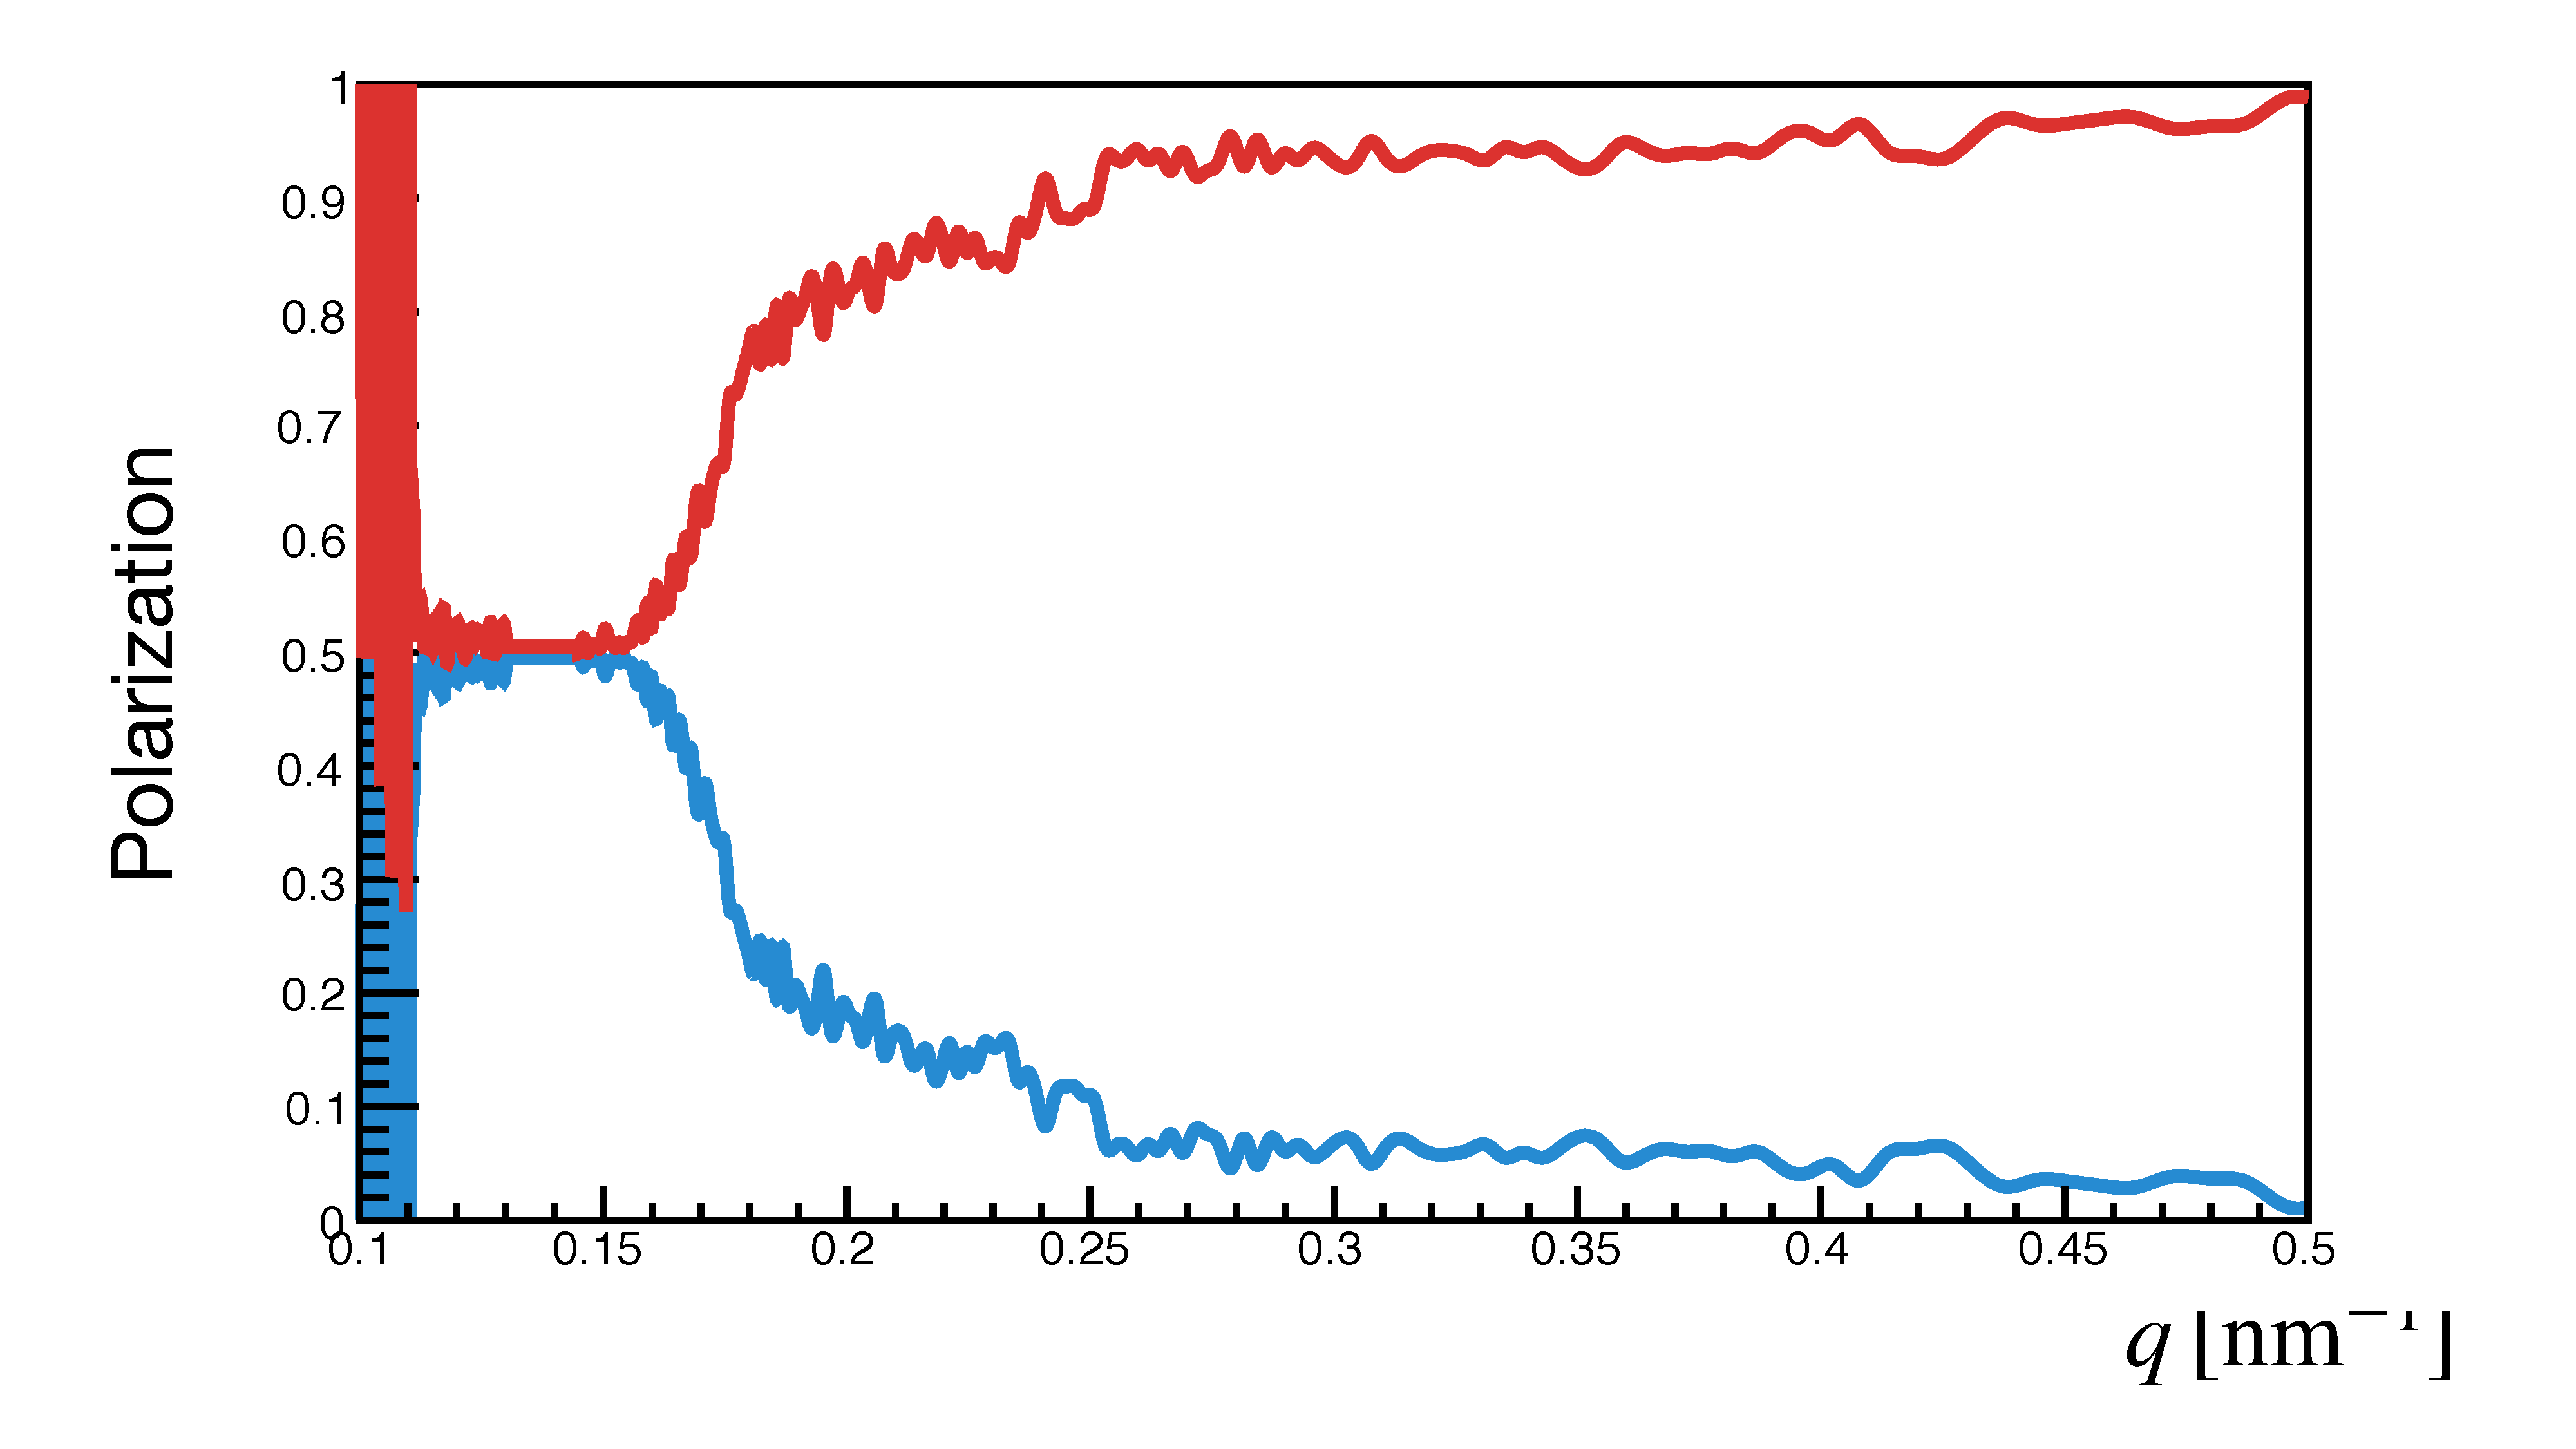
\includegraphics[width=80mm]{base.pdf}
 \caption{Model for estimating the spin up fraction (blue) and spin down fraction (red) of a neutron beam reflected by a supermirror using the spline function.}
\end{figure}


\subsubsection{Reflectmetory of polarization films}
(fig,12)のように偏極された中性子ビームを用いて、偏極解析膜の反射率を測定した。全体のセットアップを(fig,13)に示した。中性子ビームを偏極ミラーに対して$10\,\rm mrad$で入射させ、反射したビームを、横$0.1\,\rm mm$、にコリメートし、を$12\,\rm mrad$の入射角で試料(偏極解析膜)に入射し、下流 の RPMT で反射波と透過波の両方を検出した。
入射強度をダイレクト測定(試料を置かない測定)によって決定し、偏極解析膜による反射率を導出した。(fig,14)

\begin{figure}[tbh]
 \centering
 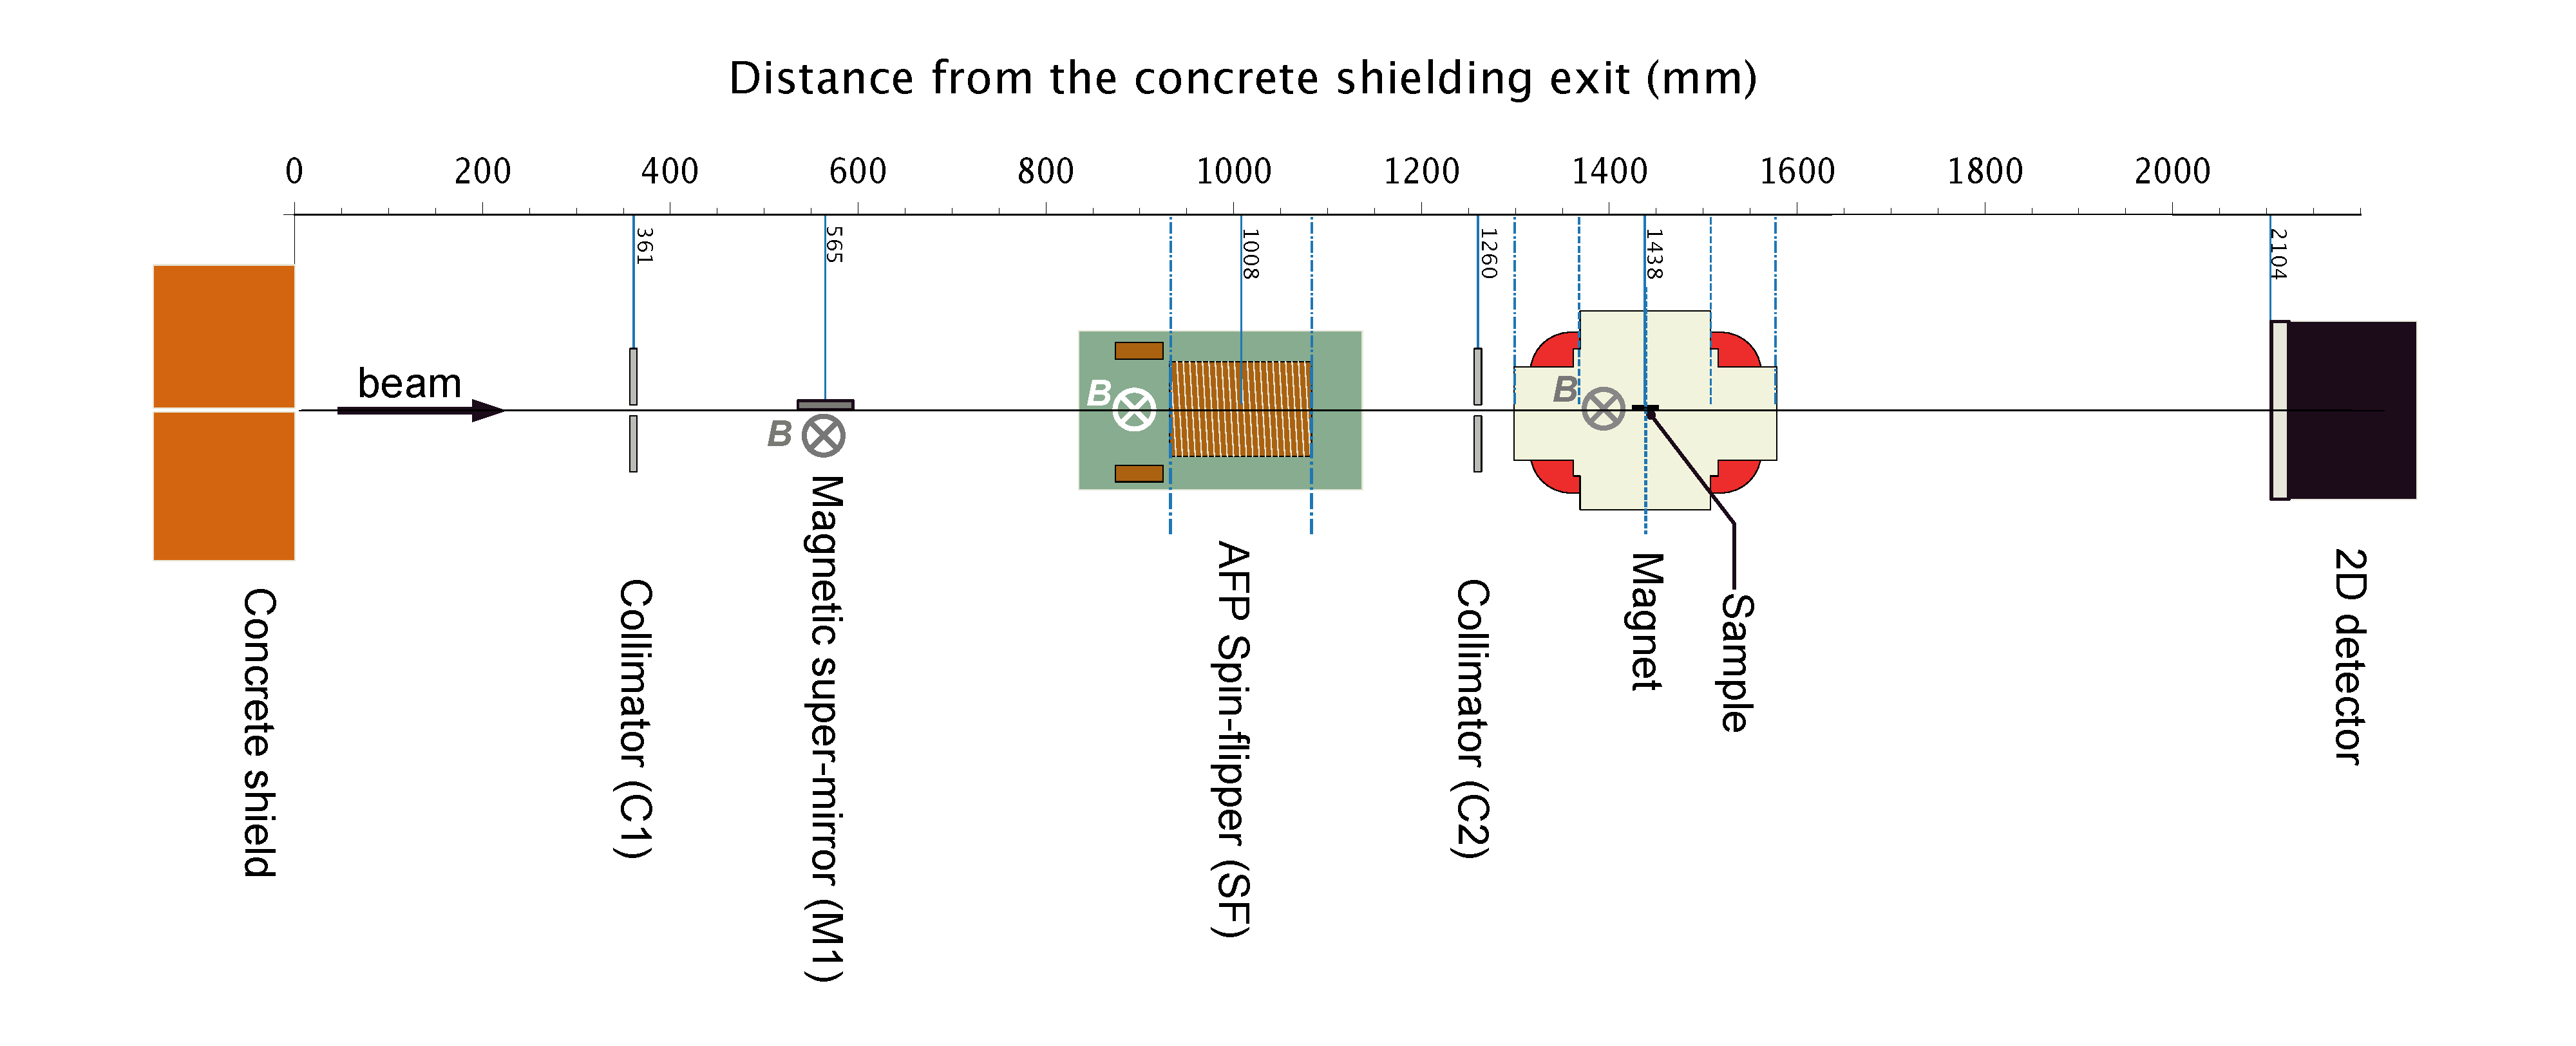
\includegraphics[width=130mm]{BL05_2.pdf}
 \caption{Neutron reflectmetory setup}
\end{figure}

試料による中性子の反射率は理論式により次のように表すことができる。

$E>V_{\rm Fe}$の時、
\begin{equation}
R=\frac{(k_0k_1-k_1k_2)^2\cos^2(k_1d)+(k_0k_2-k_1^2)^2\sin^2 (k_1d)}{(k_0k_1+k_1k_2)^2\cos^2(k_1d)+(k_0k_2+k_1^2)^2\sin^2 (k_1d)}
\end{equation}

$V_{\rm Fe}>E>V_{\rm Si}$の時、
\begin{equation}
R=\frac{(\alpha k_0-\alpha k_2)^2\cosh^2(\alpha d)+(k_0k_2+\alpha^2)^2\sinh^2 (\alpha d)}{(\alpha k_0+\alpha k_2)^2\cosh^2(\alpha d)+(\alpha^2-k_0k_2)^2\sinh^2 (\alpha d)}
\end{equation}

$E<V_{\rm Si}$の時、
\begin{equation}
R=1
\end{equation}

ここで、$k_0=\frac {\sqrt{2m_nE} }{\hbar},\,k_1=\frac {\sqrt{2m(E-V)} }{\hbar},\,k_2=\frac {\sqrt{2m(E-V_{\rm Si})} }{\hbar},\,\alpha=\frac {\sqrt{2m(V-E)} }{\hbar},\,$は中性子の波数、$m_n$は中性子の質量、$V$は中性子が感じるフェルミポテンシャル、$V_{\rm Si}$はSiのフェルミポテンシャル、$d$は鉄薄膜の厚みを表す。中性子が感じるポテンシャル$V=V_{\rm Fe}\pm \mu_n B$は、鉄のフェルミポテンシャル$V_{\rm Fe}$、中性子の磁気モーメント$\mu_n$、鉄の内部磁場$B$によって表される。上記の式で$V_{\rm Fe},\,B$ をパラメータとして実験結果をフィッティングすると、$=V_{\rm Fe}=197(1)\,\rm neV,\,B=2.17(1)\,\rm T,\,d=94.8(4)\,\rm nm$となった。(fig.15)よって、中性子のスピンが鉄薄膜の磁化した方向と平行な時のポテンシャル$V_{\rm Fe,antiparallel}$は、$V_{\rm Fe,parallel}=328(1)\,\rm neV$、反平行な時のポテンシャル$V_{\rm Fe,antiparallel}$は、$V_{\rm Fe,antiparallel}=66(1)\,\rm neV$となる。


\begin{comment}
\begin{equation}
k_0=\frac {\sqrt{2m_nE} }{\hbar}
\end{equation}

\begin{equation}
k_1=\frac {\sqrt{2m(E-V_{\rm Fe})} }{\hbar}
\end{equation}

\begin{equation}
k_2=\frac {\sqrt{2m(E-V_{\rm Si})} }{\hbar}
\end{equation}
\end{comment}

\begin{figure}[tbh]
 \centering
 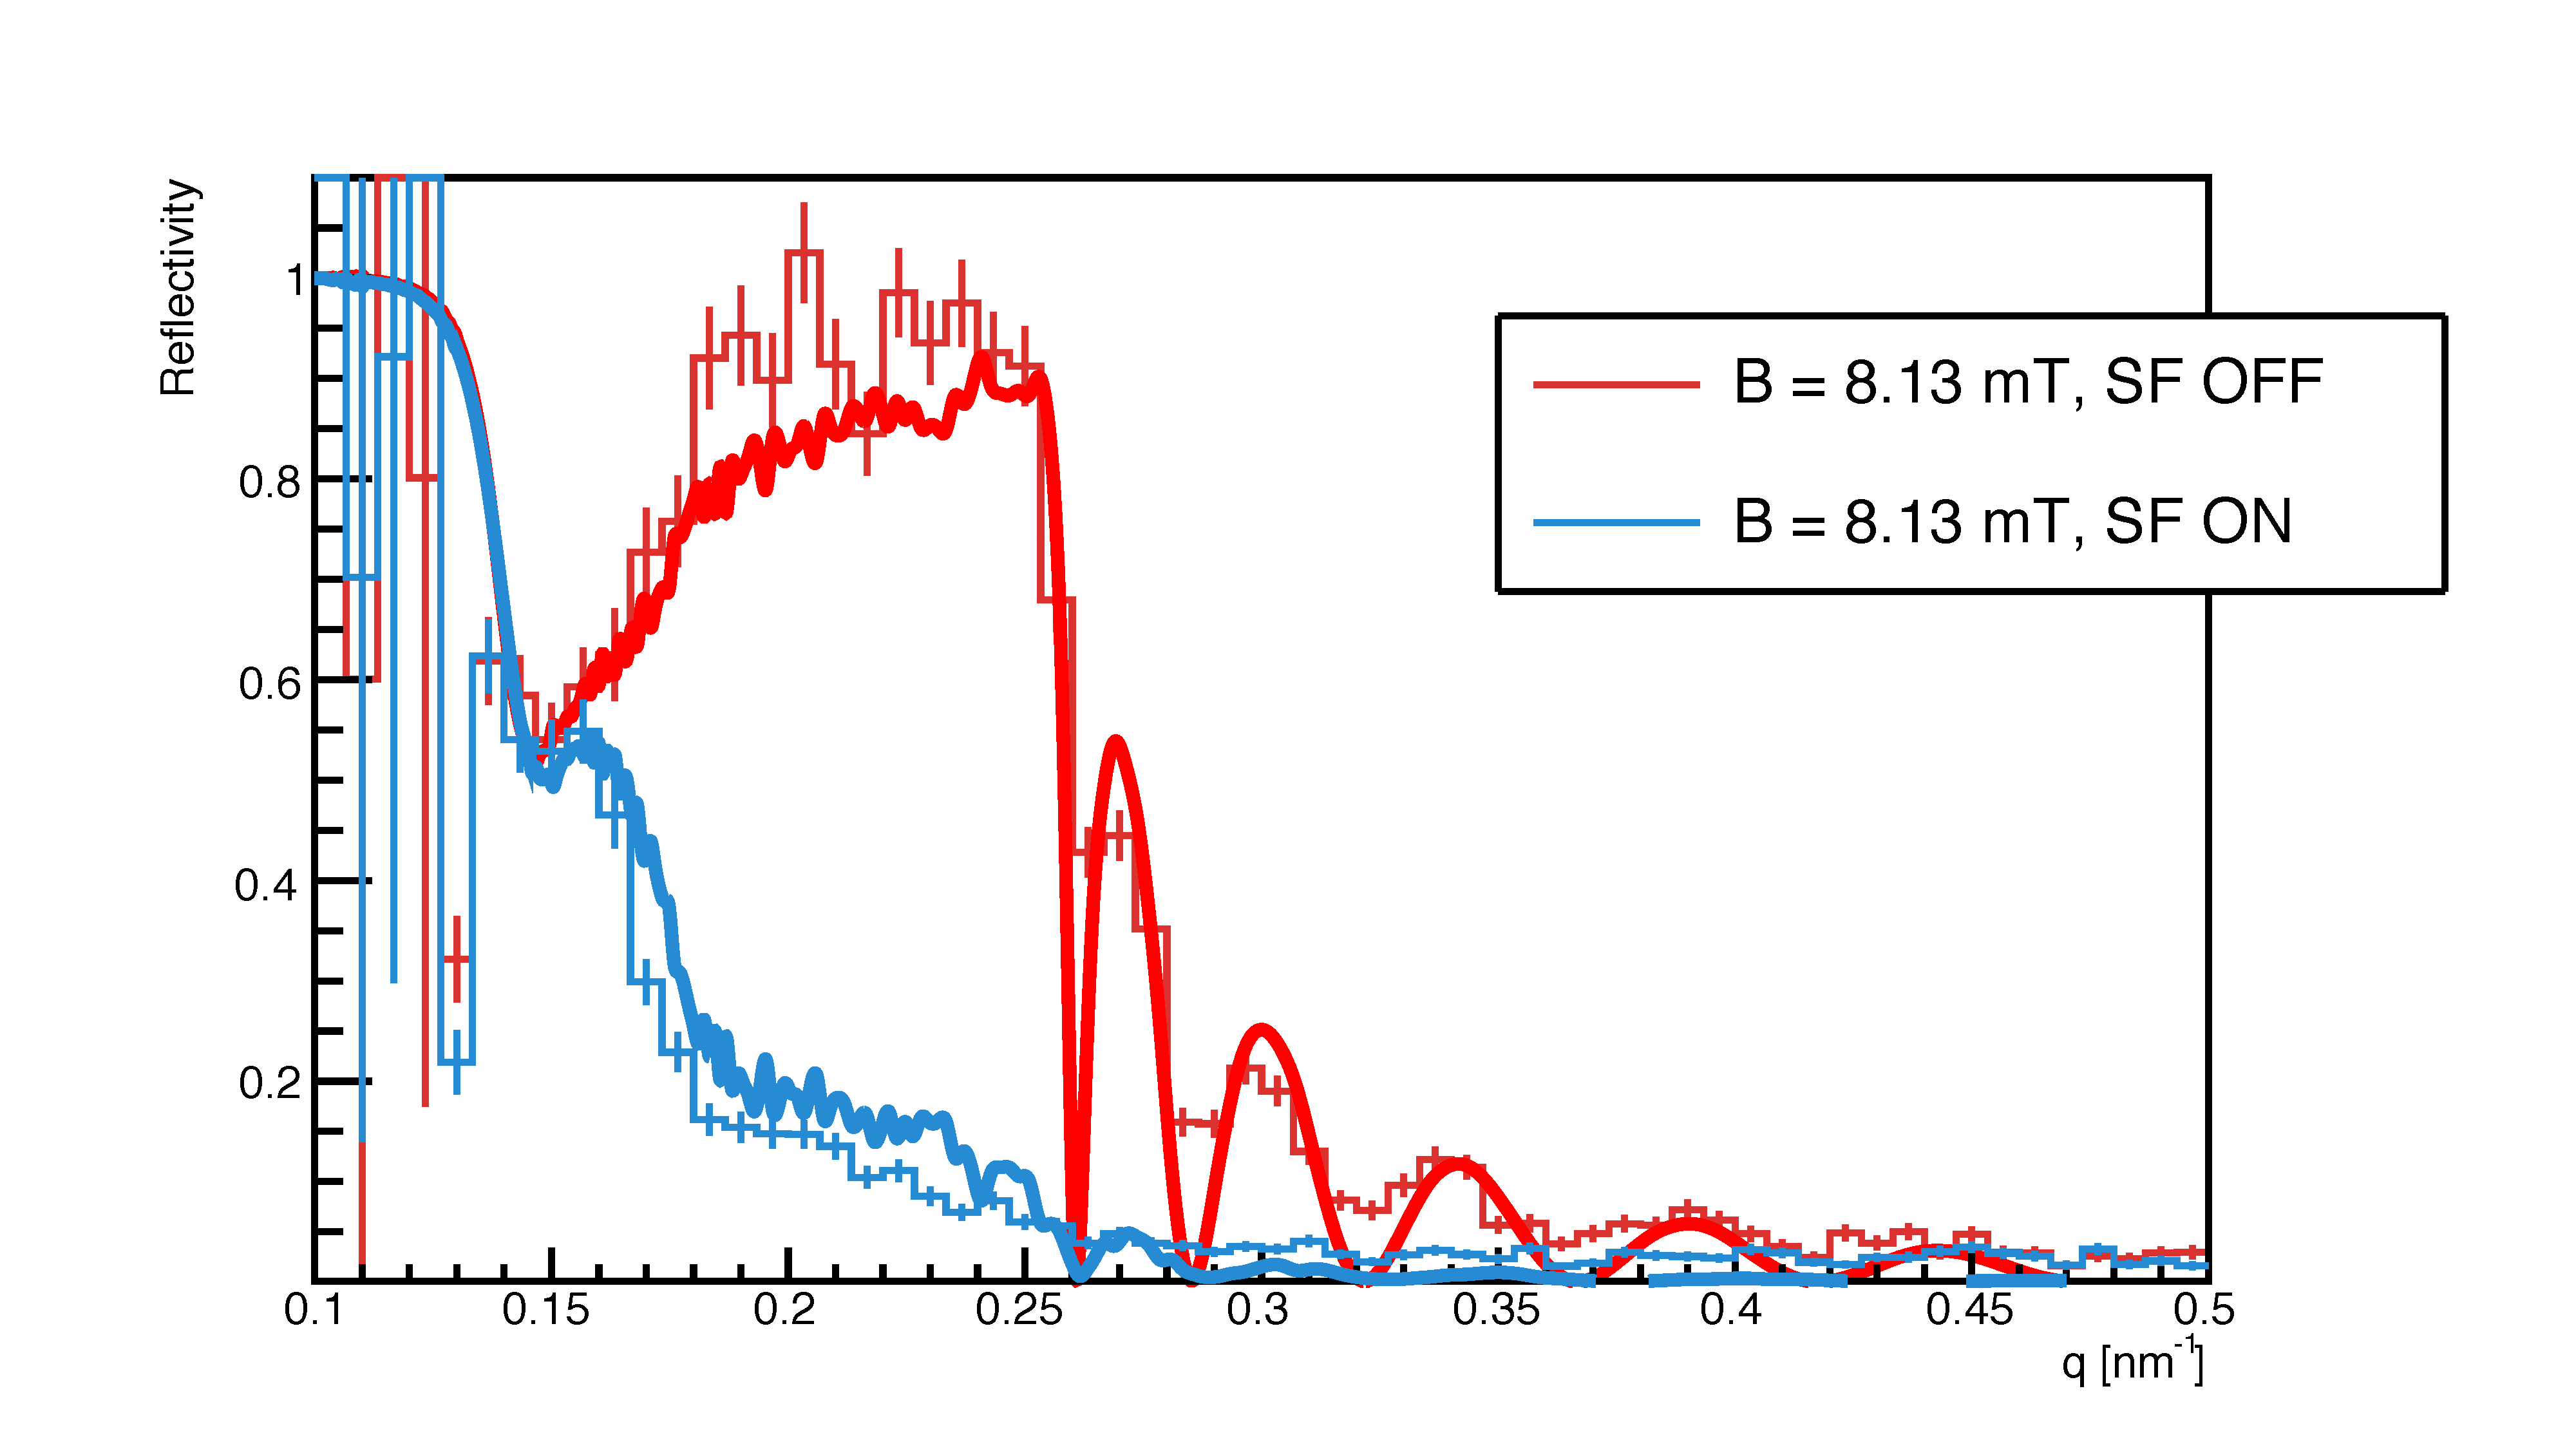
\includegraphics[width=80mm]{reflectivity.pdf}
 \caption{Neutron reflectivity of spin up(blue), spin down(red) and fitting curve of $\rm Fe$ 90 nm on a silicon substrate.}
\end{figure}

%\subsubsection{}

\section{Conclusions and Outlook}
UCNをスピン解析するための鉄薄膜の磁気特性の評価を行なった。鉄薄膜への要求は次の2点、1) 十分小さい印加磁場($\sim 15\rm\,mT$)で飽和すること。2) スピン状態が異なる中性子が感じるポテンシャル差が十分に大きいこと($\sim 2\rm\,T$)。1)はVSM測定によって、($\sim 15\rm\,mT$)で飽和することが確認された。2)は冷中性子反射率測定から、スピン状態の異なる中性子が感じるポテンシャルの大きさが、それぞれ$V_{\rm Fe,parallel}=328(1)\,\rm neV$、$V_{\rm Fe,antiparallel}=66(1)\,\rm neV$となることが分かり、十分大きなポテンシャル差$(\sim 200\,\rm neV???)$が確認された。よって、我々は十分な性能の偏極解析膜の開発に成功した。今後は2022年の春にUCNを用いた反射率測定を行い、より正確な偏極解析膜の評価が計画されている。

%\section{参考文献}
\begin{comment}

http://www.jahep.org/hepnews/2018/18-1-2-TUCAN.pdf

https://www.jstage.jst.go.jp/article/hamon/30/1/30_45/_pdf/-char/ja

https://www.jstage.jst.go.jp/article/hamon/29/1/29_22/_pdf/-char/ja

https://www.jstage.jst.go.jp/article/hamon/19/1/19_34/_pdf/-char/ja

https://www.jstage.jst.go.jp/article/jsssj/33/5/33_272/_pdf

https://www.jstage.jst.go.jp/article/electrochemistry/84/7/84_16-7-FE0052/_pdf/-char/ja

\end{comment}
\begin{comment}

質問
・abstで述べていた、先行研究よりも小さいとかの話題は入れるべき?


S. Afach et al, Euro Phys J. A \textbf{51}, 143 (2015)

\section*{方針}




・1章分増やして、KUR, JPARC分ける
・イントロが長いので短くする
・

まず目次を作る
section subsection を先に埋めてしまう
セクションの初めにメインの内容を書く「この章ではこのようなことを説明します」
cloudlatex
絵を先に入れる
次のミーティングまで
・VSM X線(膜の準備に含む)
・偏極度測定
・反射率

google scholar ""で囲って用例を調べてみる
論文の書き方を見てみる
樋口さんが送ってくれたもの


本稿はレポートのテンプレートである.

まずはじめに参考文献を引用する\cite{Knuth86}.

さらにもうひとつ引用する\cite{BollenHHJ07}.

日本語の文献も引用する\cite{Okumura07}.

最後にウェブページを引用する\cite{Github}.

\section*{表や図の描画方法}

図は\figref{sample},表は\tabref{sample}として参照する.


\begin{table}[tbh]
 \centering
 \begin{tabular}{|l|r|} \hline
 A1 & B1 \\
 A2 & B2 \\ \hline
 \end{tabular}
 \caption{図の参考例}
 \tablab{sample}
\end{table}

\section{おわりに}

本稿において本文を通してレポートの執筆が可能な環境であることが示された.
\end{comment}


\begin{thebibliography}{99}
  \bibitem{PSI}  C. Abel et al., Phys. Rev. Lett. \textbf{124}, 081803 (2020). 
  \bibitem{Ramsey} N. F. Ramsey, Phys. Rev.\textbf{78}, 695 (1950).
 
  \bibitem{Hino} M. Hino et al, Nucl. Inst. Meth. A \textbf{797}, 265 (2015)
  \bibitem{SSA}S. Afach, et al, Euro. Phys. Jour. A 51, 143 (2015) 
  %\bibitem{}
  
\end{thebibliography}

\end{document}